% =====================================================================
% CHUONG 3 - DU LIEU VA TIEN XU LY DU LIEU
% Tac gia: Pham The Duc (Data Engineer & Data Analyst)
% Cach dung: copy thu muc figures/ vao project Overleaf, roi them
%   % =====================================================================
% CHUONG 3 - DU LIEU VA TIEN XU LY DU LIEU
% Tac gia: Pham The Duc (Data Engineer & Data Analyst)
% Cach dung: copy thu muc figures/ vao project Overleaf, roi them
%   % =====================================================================
% CHUONG 3 - DU LIEU VA TIEN XU LY DU LIEU
% Tac gia: Pham The Duc (Data Engineer & Data Analyst)
% Cach dung: copy thu muc figures/ vao project Overleaf, roi them
%   % =====================================================================
% CHUONG 3 - DU LIEU VA TIEN XU LY DU LIEU
% Tac gia: Pham The Duc (Data Engineer & Data Analyst)
% Cach dung: copy thu muc figures/ vao project Overleaf, roi them
%   \input{chuong3}
% vao main.tex. Yeu cau goi cac package: graphicx, booktabs.
% Neu dung documentclass{article}, doi \chapter -> \section.
% =====================================================================

\chapter{Dữ liệu và tiền xử lý dữ liệu}
\label{chap:data}

\section{Giới thiệu bộ dữ liệu}
Bộ dữ liệu sử dụng là \textbf{Heart Disease Dataset} trên Kaggle
(\texttt{johnsmith88/heart-disease-dataset}), tổng hợp từ bốn cơ sở dữ liệu y tế
(Cleveland, Hungary, Switzerland, Long Beach V) từ năm 1988. Tuy bản gốc có 76
thuộc tính, các nghiên cứu công bố đều sử dụng tập con gồm \textbf{14 thuộc tính}.

\begin{itemize}
  \item Số bản ghi ban đầu: 1025 dòng.
  \item Số thuộc tính: 13 đặc trưng đầu vào và 1 biến mục tiêu \texttt{target}.
  \item Bài toán: phân loại nhị phân, dự đoán bệnh nhân \emph{có nguy cơ}
        (\texttt{target = 1}) hay \emph{không} (\texttt{target = 0}).
\end{itemize}

\begin{table}[h]
\centering
\caption{Mô tả các thuộc tính của bộ dữ liệu}
\label{tab:attributes}
\begin{tabular}{cllc}
\toprule
\# & Thuộc tính & Ý nghĩa & Kiểu \\
\midrule
1  & \texttt{age}      & Tuổi (năm)                              & Liên tục \\
2  & \texttt{sex}      & Giới tính (1 = nam, 0 = nữ)             & Nhị phân \\
3  & \texttt{cp}       & Kiểu đau ngực (0--3)                    & Phân loại \\
4  & \texttt{trestbps} & Huyết áp lúc nghỉ (mm Hg)               & Liên tục \\
5  & \texttt{chol}     & Cholesterol huyết thanh (mg/dl)         & Liên tục \\
6  & \texttt{fbs}      & Đường huyết đói $>$ 120 mg/dl (1/0)     & Nhị phân \\
7  & \texttt{restecg}  & Điện tâm đồ lúc nghỉ (0--2)             & Phân loại \\
8  & \texttt{thalach}  & Nhịp tim tối đa đạt được                & Liên tục \\
9  & \texttt{exang}    & Đau thắt ngực khi gắng sức (1/0)        & Nhị phân \\
10 & \texttt{oldpeak}  & Độ chênh đoạn ST khi gắng sức           & Liên tục \\
11 & \texttt{slope}    & Độ dốc đoạn ST khi gắng sức (0--2)      & Phân loại \\
12 & \texttt{ca}       & Số mạch máu lớn nhuộm màu (0--4)        & Phân loại \\
13 & \texttt{thal}     & Tình trạng thalassemia (0--3)           & Phân loại \\
14 & \texttt{target}   & Nhãn: 1 = có nguy cơ, 0 = không         & Nhị phân \\
\bottomrule
\end{tabular}
\end{table}

\section{Thống kê mô tả}
Các đặc trưng liên tục có thang đo rất khác nhau: \texttt{chol} ở mức hàng trăm
(126--564) trong khi \texttt{oldpeak} chỉ dao động 0--6.2. Do đó cần
\textbf{chuẩn hoá} trước khi đưa vào mạng nơ-ron (mục~\ref{sec:fe}).

\section{Kiểm tra chất lượng dữ liệu}

\subsection{Giá trị thiếu}
Kiểm tra bằng \texttt{df.isnull().sum()}: \textbf{không có ô thiếu}.

\subsection{Bản ghi trùng lặp}
Kiểm tra bằng \texttt{df.duplicated().sum()} cho thấy trong 1025 bản ghi có
\textbf{723 bản trùng lặp hoàn toàn}, chỉ còn \textbf{302 bản ghi duy nhất}.
Nếu giữ lại, một bệnh nhân có thể xuất hiện đồng thời ở cả tập train và test,
gây \textbf{rò rỉ dữ liệu (data leakage)} làm độ chính xác bị cao giả tạo. Vì
vậy nhóm loại bỏ toàn bộ bản trùng trước khi chia dữ liệu.

\subsection{Giá trị ngoại lệ (Outlier)}
Áp dụng quy tắc \textbf{IQR}: giá trị ngoài khoảng
$[Q_1 - 1.5\,\mathrm{IQR},\; Q_3 + 1.5\,\mathrm{IQR}]$ được coi là ngoại lệ.
Các outlier ở \texttt{trestbps}, \texttt{chol}, \texttt{thalach},
\texttt{oldpeak} được \textbf{cắt về biên} (winsorize) nhằm giảm nhiễu mà vẫn
giữ lại bản ghi.

\subsection{Giá trị bất thường về mã hoá}
\texttt{ca} có giá trị 4 và \texttt{thal} có giá trị 0 nằm ngoài bảng mã chuẩn;
do số lượng nhỏ, chúng được giữ lại như một mức phân loại riêng.

\section{Tiền xử lý dữ liệu}
Quy trình trong \texttt{src/data\_preprocessing.py}:
\begin{enumerate}
  \item Đọc dữ liệu thô \texttt{data/raw/heart.csv}.
  \item Loại bản ghi trùng: $1025 \rightarrow 302$ dòng.
  \item Điền giá trị thiếu (nếu có): liên tục dùng trung vị, phân loại dùng mode.
  \item Chuẩn hoá kiểu dữ liệu: cột phân loại/nhị phân về \texttt{int}, liên tục
        về \texttt{float}.
  \item Xử lý outlier bằng cách cắt về biên IQR.
  \item Lưu \texttt{data/processed/heart\_clean.csv} (302 dòng $\times$ 14 cột).
\end{enumerate}

\section{Feature Engineering}
\label{sec:fe}
Cài đặt trong \texttt{src/feature\_engineering.py}:
\begin{itemize}
  \item Mã hoá biến phân loại bằng \texttt{LabelEncoder} (giữ nguyên 13 đặc trưng
        để khớp lớp \texttt{Input(13)} của mô hình ANN).
  \item Chuẩn hoá đặc trưng liên tục bằng \texttt{StandardScaler} (trung bình 0,
        độ lệch chuẩn 1).
  \item Chống rò rỉ dữ liệu: \texttt{StandardScaler} chỉ \texttt{fit} trên tập
        train rồi áp dụng cho cả train và test; scaler được lưu tại
        \texttt{saved\_models/scaler.pkl}.
\end{itemize}

\section{Chia tập dữ liệu train/test}
Sử dụng \texttt{train\_test\_split()} với tỷ lệ \textbf{80\% train -- 20\% test},
\texttt{stratify} theo nhãn và \texttt{random\_state = 42}.

\begin{table}[h]
\centering
\caption{Kết quả chia tập dữ liệu}
\label{tab:split}
\begin{tabular}{lccc}
\toprule
Tập & Số mẫu & Nhãn 1 (có bệnh) & Nhãn 0 (không bệnh) \\
\midrule
Train & 241 & 131 & 110 \\
Test  & 61  & 33  & 28  \\
\midrule
Tổng  & 302 & 164 & 138 \\
\bottomrule
\end{tabular}
\end{table}

Kết quả lưu thành \texttt{data/processed/train.csv} và
\texttt{data/processed/test.csv}.

\section{Phân tích dữ liệu khám phá (EDA)}
EDA được thực hiện trong \texttt{notebook/data\_exploration.ipynb}.

\begin{figure}[h]
  \centering
  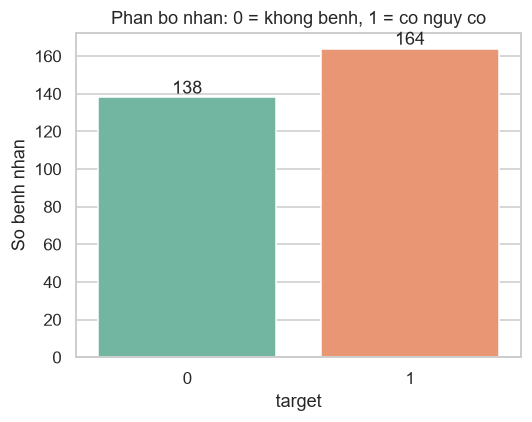
\includegraphics[width=0.5\textwidth]{figures/target_distribution.png}
  \caption{Phân bố biến mục tiêu \texttt{target} (cân bằng $\approx$ 54\%/46\%).}
  \label{fig:target}
\end{figure}

\begin{figure}[h]
  \centering
  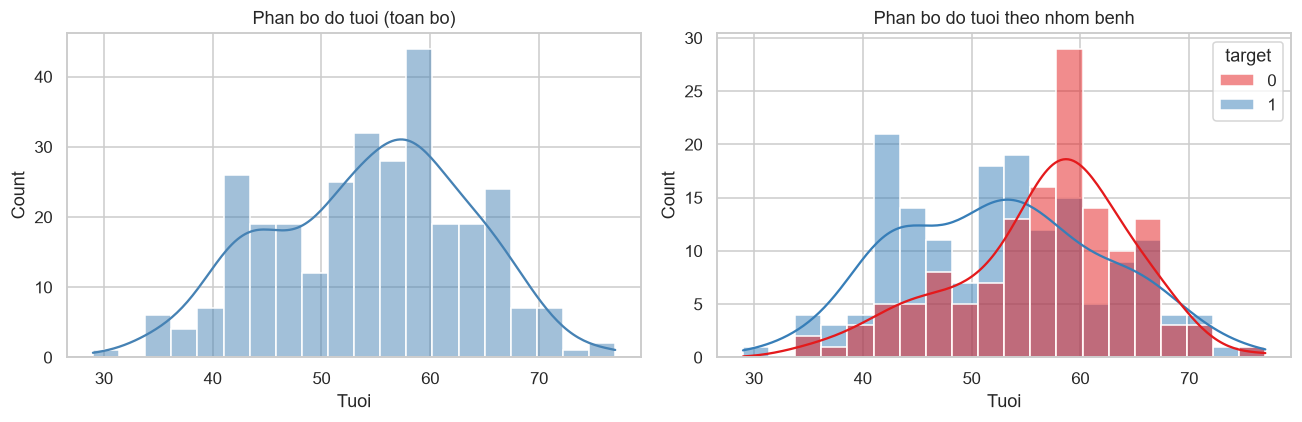
\includegraphics[width=\textwidth]{figures/age_distribution.png}
  \caption{Phân bố độ tuổi theo toàn bộ và theo nhóm bệnh.}
  \label{fig:age}
\end{figure}

\begin{figure}[h]
  \centering
  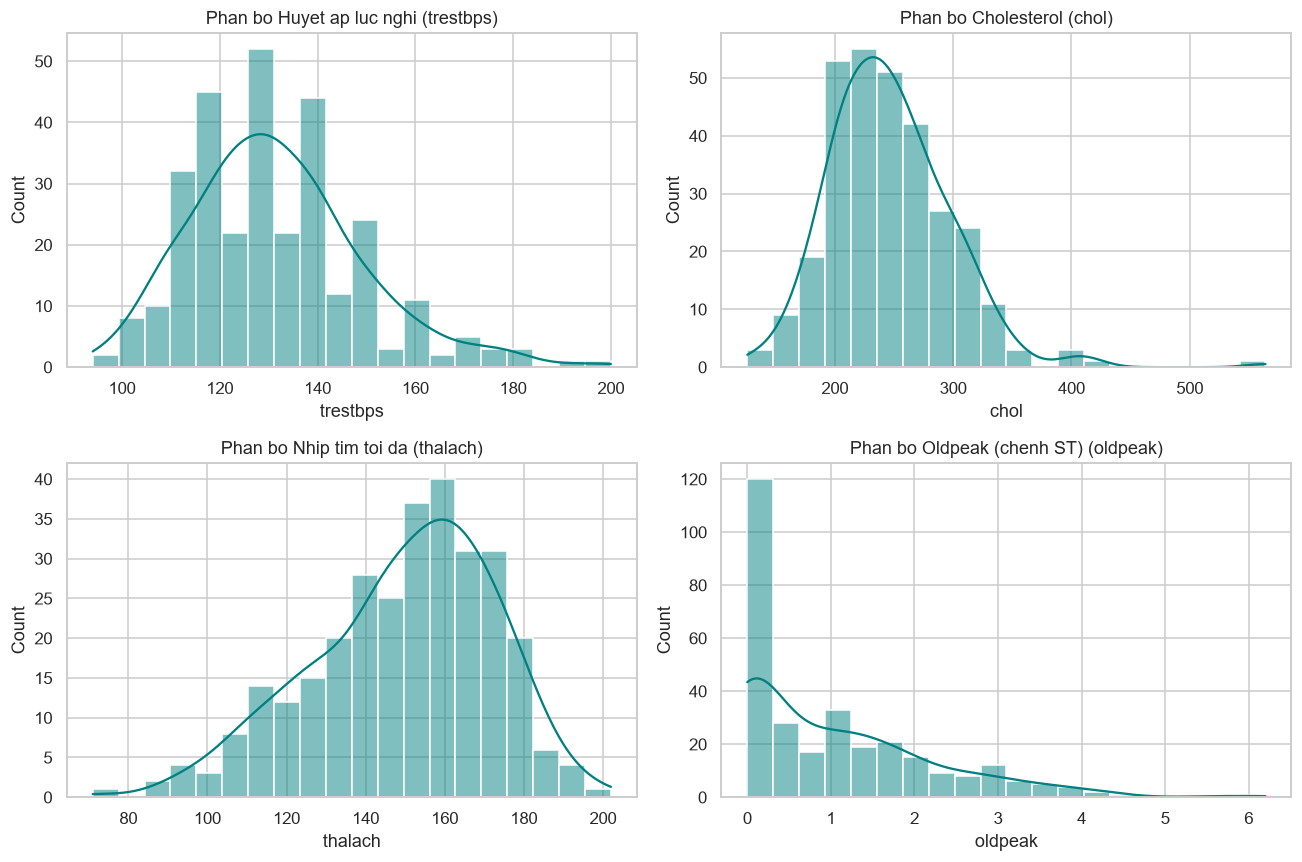
\includegraphics[width=\textwidth]{figures/continuous_histograms.png}
  \caption{Histogram các đặc trưng liên tục.}
  \label{fig:hist}
\end{figure}

\begin{figure}[h]
  \centering
  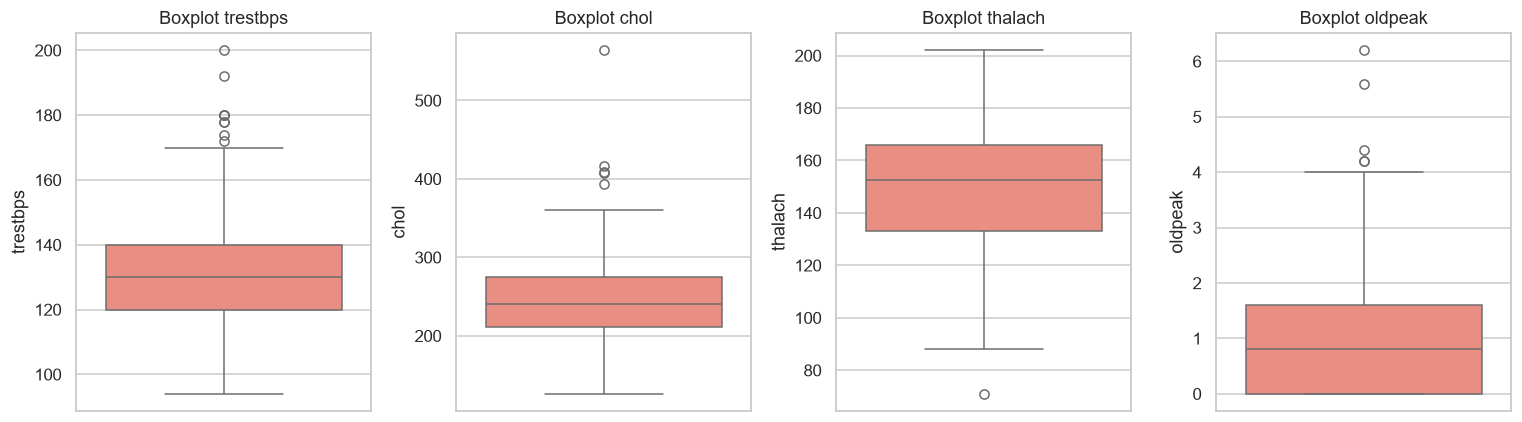
\includegraphics[width=\textwidth]{figures/continuous_boxplots.png}
  \caption{Boxplot các đặc trưng liên tục (quan sát outlier).}
  \label{fig:box}
\end{figure}

\begin{figure}[h]
  \centering
  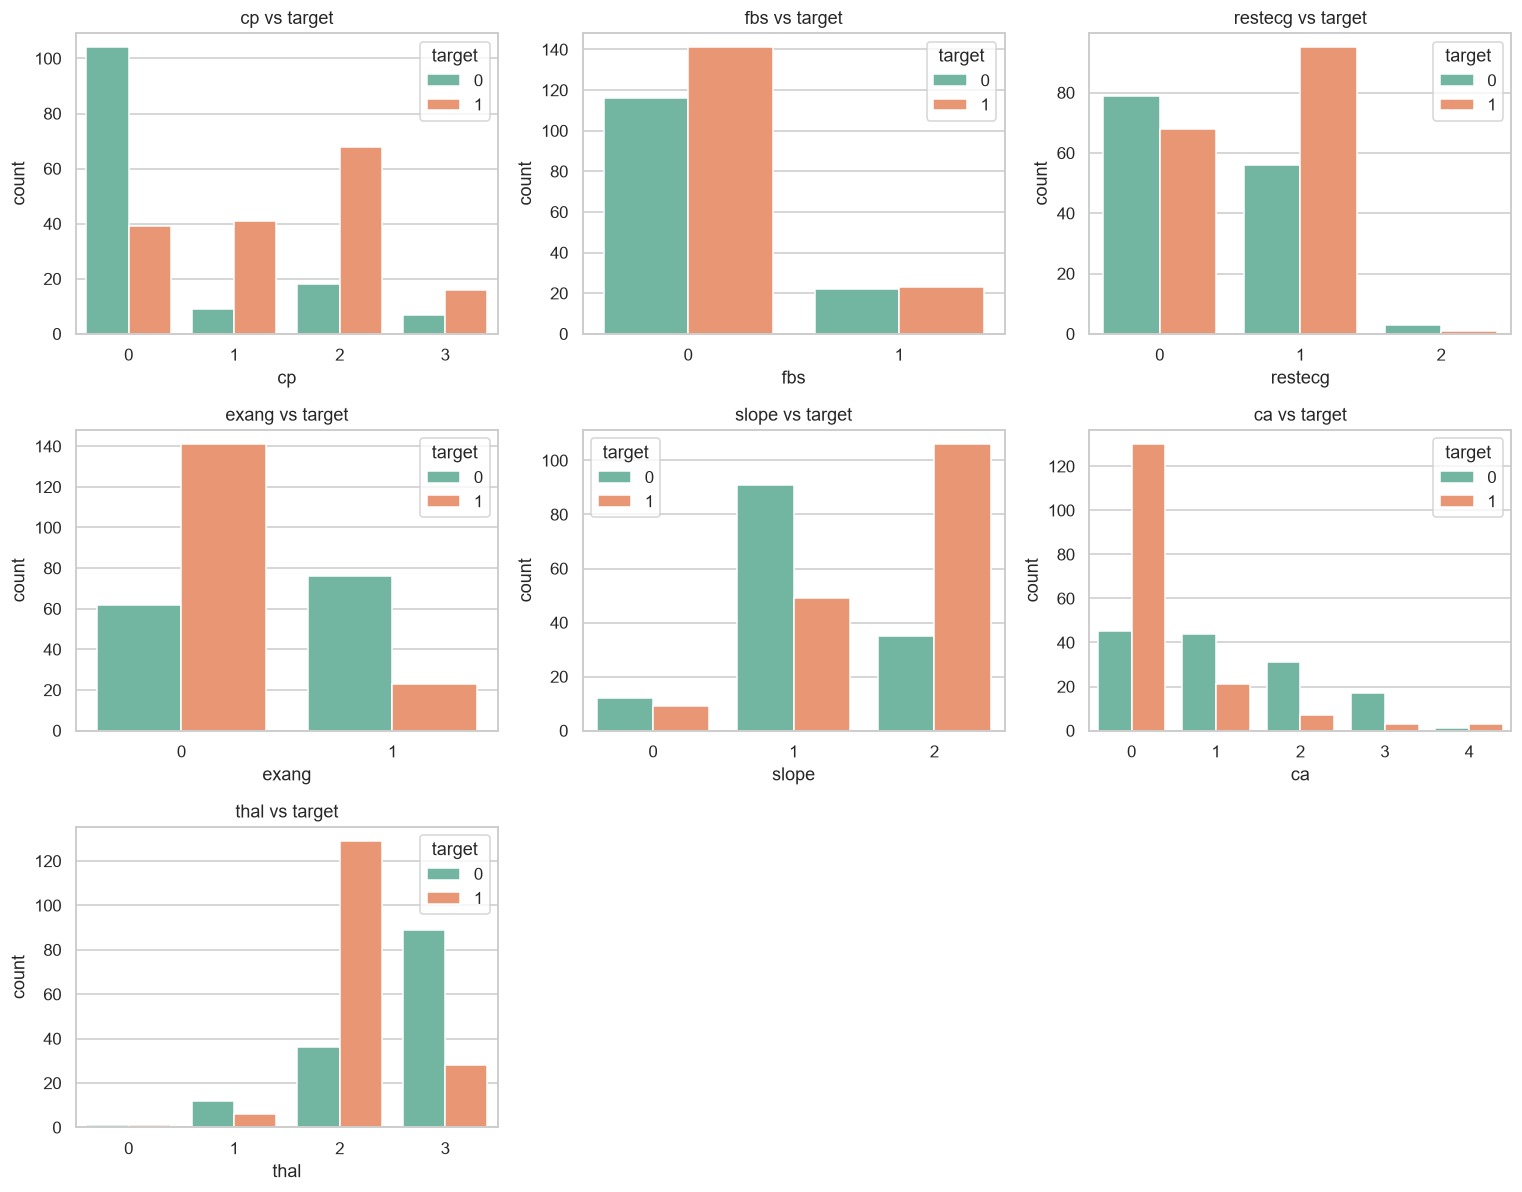
\includegraphics[width=\textwidth]{figures/categorical_countplots.png}
  \caption{Countplot các biến phân loại theo nhãn.}
  \label{fig:cat}
\end{figure}

\begin{figure}[h]
  \centering
  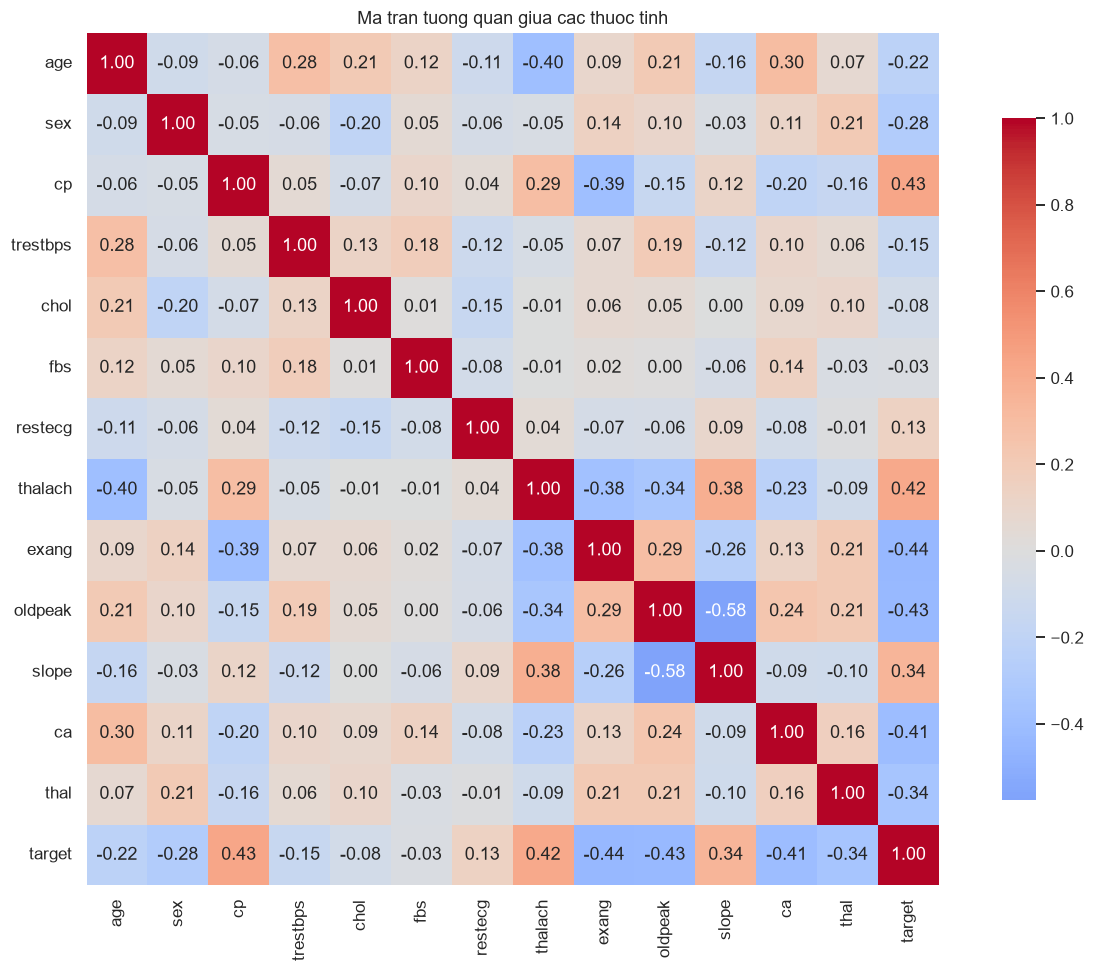
\includegraphics[width=0.9\textwidth]{figures/correlation_heatmap.png}
  \caption{Ma trận tương quan giữa các thuộc tính.}
  \label{fig:corr}
\end{figure}

\begin{table}[h]
\centering
\caption{Tương quan của từng thuộc tính với \texttt{target} (sắp theo độ lớn)}
\label{tab:corr}
\begin{tabular}{lc lc}
\toprule
Thuộc tính & Hệ số & Thuộc tính & Hệ số \\
\midrule
\texttt{exang}   & $-0.436$ & \texttt{thal}     & $-0.343$ \\
\texttt{cp}      & $+0.432$ & \texttt{sex}      & $-0.284$ \\
\texttt{oldpeak} & $-0.429$ & \texttt{age}      & $-0.221$ \\
\texttt{thalach} & $+0.420$ & \texttt{trestbps} & $-0.146$ \\
\texttt{ca}      & $-0.409$ & \texttt{restecg}  & $+0.135$ \\
\texttt{slope}   & $+0.344$ & \texttt{chol}     & $-0.081$ \\
                 &          & \texttt{fbs}      & $-0.027$ \\
\bottomrule
\end{tabular}
\end{table}

\textbf{Nhận xét:} các thuộc tính tương quan mạnh nhất với nguy cơ bệnh tim là
\texttt{exang}, \texttt{cp}, \texttt{oldpeak}, \texttt{thalach}, \texttt{ca},
phù hợp với y văn. Hai thuộc tính \texttt{chol} và \texttt{fbs} tương quan yếu
nhất với nhãn.

\section{Kết luận chương}
Chương 3 đã hoàn thành khâu chuẩn bị dữ liệu: làm sạch (loại 723 bản trùng còn
302 dòng, không có giá trị thiếu, xử lý outlier), chuẩn hoá đặc trưng bằng
\texttt{StandardScaler} (fit trên train để tránh rò rỉ dữ liệu), chia dữ liệu
80/20 có phân tầng và xuất \texttt{train.csv}/\texttt{test.csv}. EDA cho thấy dữ
liệu cân bằng nhãn và xác định được nhóm đặc trưng quan trọng. Bộ dữ liệu đã sẵn
sàng cho Chương 4 -- thiết kế và huấn luyện mô hình ANN.

% vao main.tex. Yeu cau goi cac package: graphicx, booktabs.
% Neu dung documentclass{article}, doi \chapter -> \section.
% =====================================================================

\chapter{Dữ liệu và tiền xử lý dữ liệu}
\label{chap:data}

\section{Giới thiệu bộ dữ liệu}
Bộ dữ liệu sử dụng là \textbf{Heart Disease Dataset} trên Kaggle
(\texttt{johnsmith88/heart-disease-dataset}), tổng hợp từ bốn cơ sở dữ liệu y tế
(Cleveland, Hungary, Switzerland, Long Beach V) từ năm 1988. Tuy bản gốc có 76
thuộc tính, các nghiên cứu công bố đều sử dụng tập con gồm \textbf{14 thuộc tính}.

\begin{itemize}
  \item Số bản ghi ban đầu: 1025 dòng.
  \item Số thuộc tính: 13 đặc trưng đầu vào và 1 biến mục tiêu \texttt{target}.
  \item Bài toán: phân loại nhị phân, dự đoán bệnh nhân \emph{có nguy cơ}
        (\texttt{target = 1}) hay \emph{không} (\texttt{target = 0}).
\end{itemize}

\begin{table}[h]
\centering
\caption{Mô tả các thuộc tính của bộ dữ liệu}
\label{tab:attributes}
\begin{tabular}{cllc}
\toprule
\# & Thuộc tính & Ý nghĩa & Kiểu \\
\midrule
1  & \texttt{age}      & Tuổi (năm)                              & Liên tục \\
2  & \texttt{sex}      & Giới tính (1 = nam, 0 = nữ)             & Nhị phân \\
3  & \texttt{cp}       & Kiểu đau ngực (0--3)                    & Phân loại \\
4  & \texttt{trestbps} & Huyết áp lúc nghỉ (mm Hg)               & Liên tục \\
5  & \texttt{chol}     & Cholesterol huyết thanh (mg/dl)         & Liên tục \\
6  & \texttt{fbs}      & Đường huyết đói $>$ 120 mg/dl (1/0)     & Nhị phân \\
7  & \texttt{restecg}  & Điện tâm đồ lúc nghỉ (0--2)             & Phân loại \\
8  & \texttt{thalach}  & Nhịp tim tối đa đạt được                & Liên tục \\
9  & \texttt{exang}    & Đau thắt ngực khi gắng sức (1/0)        & Nhị phân \\
10 & \texttt{oldpeak}  & Độ chênh đoạn ST khi gắng sức           & Liên tục \\
11 & \texttt{slope}    & Độ dốc đoạn ST khi gắng sức (0--2)      & Phân loại \\
12 & \texttt{ca}       & Số mạch máu lớn nhuộm màu (0--4)        & Phân loại \\
13 & \texttt{thal}     & Tình trạng thalassemia (0--3)           & Phân loại \\
14 & \texttt{target}   & Nhãn: 1 = có nguy cơ, 0 = không         & Nhị phân \\
\bottomrule
\end{tabular}
\end{table}

\section{Thống kê mô tả}
Các đặc trưng liên tục có thang đo rất khác nhau: \texttt{chol} ở mức hàng trăm
(126--564) trong khi \texttt{oldpeak} chỉ dao động 0--6.2. Do đó cần
\textbf{chuẩn hoá} trước khi đưa vào mạng nơ-ron (mục~\ref{sec:fe}).

\section{Kiểm tra chất lượng dữ liệu}

\subsection{Giá trị thiếu}
Kiểm tra bằng \texttt{df.isnull().sum()}: \textbf{không có ô thiếu}.

\subsection{Bản ghi trùng lặp}
Kiểm tra bằng \texttt{df.duplicated().sum()} cho thấy trong 1025 bản ghi có
\textbf{723 bản trùng lặp hoàn toàn}, chỉ còn \textbf{302 bản ghi duy nhất}.
Nếu giữ lại, một bệnh nhân có thể xuất hiện đồng thời ở cả tập train và test,
gây \textbf{rò rỉ dữ liệu (data leakage)} làm độ chính xác bị cao giả tạo. Vì
vậy nhóm loại bỏ toàn bộ bản trùng trước khi chia dữ liệu.

\subsection{Giá trị ngoại lệ (Outlier)}
Áp dụng quy tắc \textbf{IQR}: giá trị ngoài khoảng
$[Q_1 - 1.5\,\mathrm{IQR},\; Q_3 + 1.5\,\mathrm{IQR}]$ được coi là ngoại lệ.
Các outlier ở \texttt{trestbps}, \texttt{chol}, \texttt{thalach},
\texttt{oldpeak} được \textbf{cắt về biên} (winsorize) nhằm giảm nhiễu mà vẫn
giữ lại bản ghi.

\subsection{Giá trị bất thường về mã hoá}
\texttt{ca} có giá trị 4 và \texttt{thal} có giá trị 0 nằm ngoài bảng mã chuẩn;
do số lượng nhỏ, chúng được giữ lại như một mức phân loại riêng.

\section{Tiền xử lý dữ liệu}
Quy trình trong \texttt{src/data\_preprocessing.py}:
\begin{enumerate}
  \item Đọc dữ liệu thô \texttt{data/raw/heart.csv}.
  \item Loại bản ghi trùng: $1025 \rightarrow 302$ dòng.
  \item Điền giá trị thiếu (nếu có): liên tục dùng trung vị, phân loại dùng mode.
  \item Chuẩn hoá kiểu dữ liệu: cột phân loại/nhị phân về \texttt{int}, liên tục
        về \texttt{float}.
  \item Xử lý outlier bằng cách cắt về biên IQR.
  \item Lưu \texttt{data/processed/heart\_clean.csv} (302 dòng $\times$ 14 cột).
\end{enumerate}

\section{Feature Engineering}
\label{sec:fe}
Cài đặt trong \texttt{src/feature\_engineering.py}:
\begin{itemize}
  \item Mã hoá biến phân loại bằng \texttt{LabelEncoder} (giữ nguyên 13 đặc trưng
        để khớp lớp \texttt{Input(13)} của mô hình ANN).
  \item Chuẩn hoá đặc trưng liên tục bằng \texttt{StandardScaler} (trung bình 0,
        độ lệch chuẩn 1).
  \item Chống rò rỉ dữ liệu: \texttt{StandardScaler} chỉ \texttt{fit} trên tập
        train rồi áp dụng cho cả train và test; scaler được lưu tại
        \texttt{saved\_models/scaler.pkl}.
\end{itemize}

\section{Chia tập dữ liệu train/test}
Sử dụng \texttt{train\_test\_split()} với tỷ lệ \textbf{80\% train -- 20\% test},
\texttt{stratify} theo nhãn và \texttt{random\_state = 42}.

\begin{table}[h]
\centering
\caption{Kết quả chia tập dữ liệu}
\label{tab:split}
\begin{tabular}{lccc}
\toprule
Tập & Số mẫu & Nhãn 1 (có bệnh) & Nhãn 0 (không bệnh) \\
\midrule
Train & 241 & 131 & 110 \\
Test  & 61  & 33  & 28  \\
\midrule
Tổng  & 302 & 164 & 138 \\
\bottomrule
\end{tabular}
\end{table}

Kết quả lưu thành \texttt{data/processed/train.csv} và
\texttt{data/processed/test.csv}.

\section{Phân tích dữ liệu khám phá (EDA)}
EDA được thực hiện trong \texttt{notebook/data\_exploration.ipynb}.

\begin{figure}[h]
  \centering
  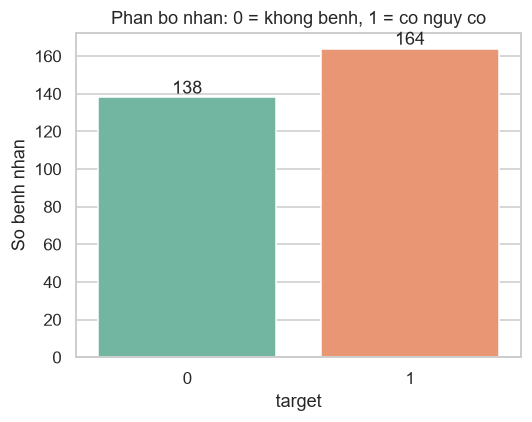
\includegraphics[width=0.5\textwidth]{figures/target_distribution.png}
  \caption{Phân bố biến mục tiêu \texttt{target} (cân bằng $\approx$ 54\%/46\%).}
  \label{fig:target}
\end{figure}

\begin{figure}[h]
  \centering
  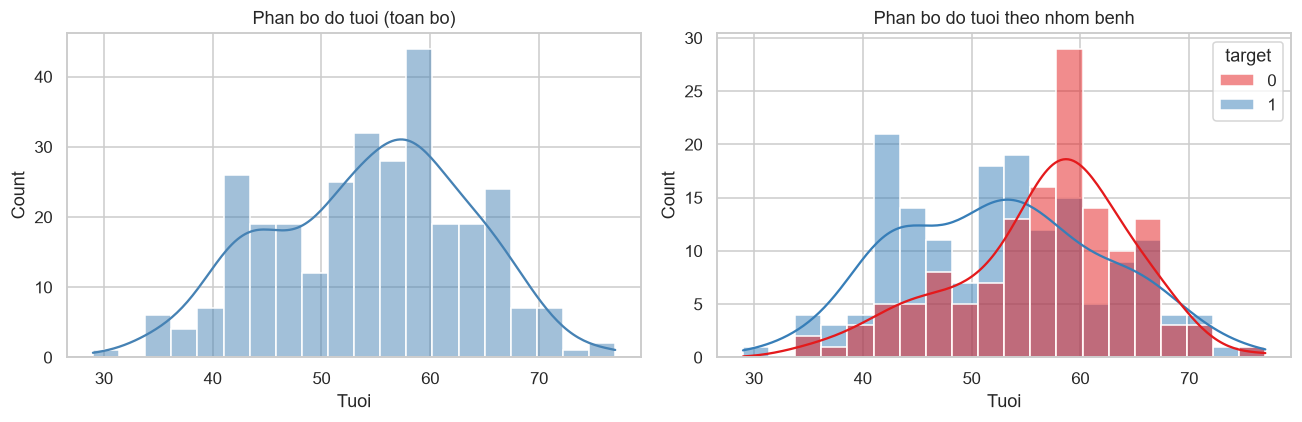
\includegraphics[width=\textwidth]{figures/age_distribution.png}
  \caption{Phân bố độ tuổi theo toàn bộ và theo nhóm bệnh.}
  \label{fig:age}
\end{figure}

\begin{figure}[h]
  \centering
  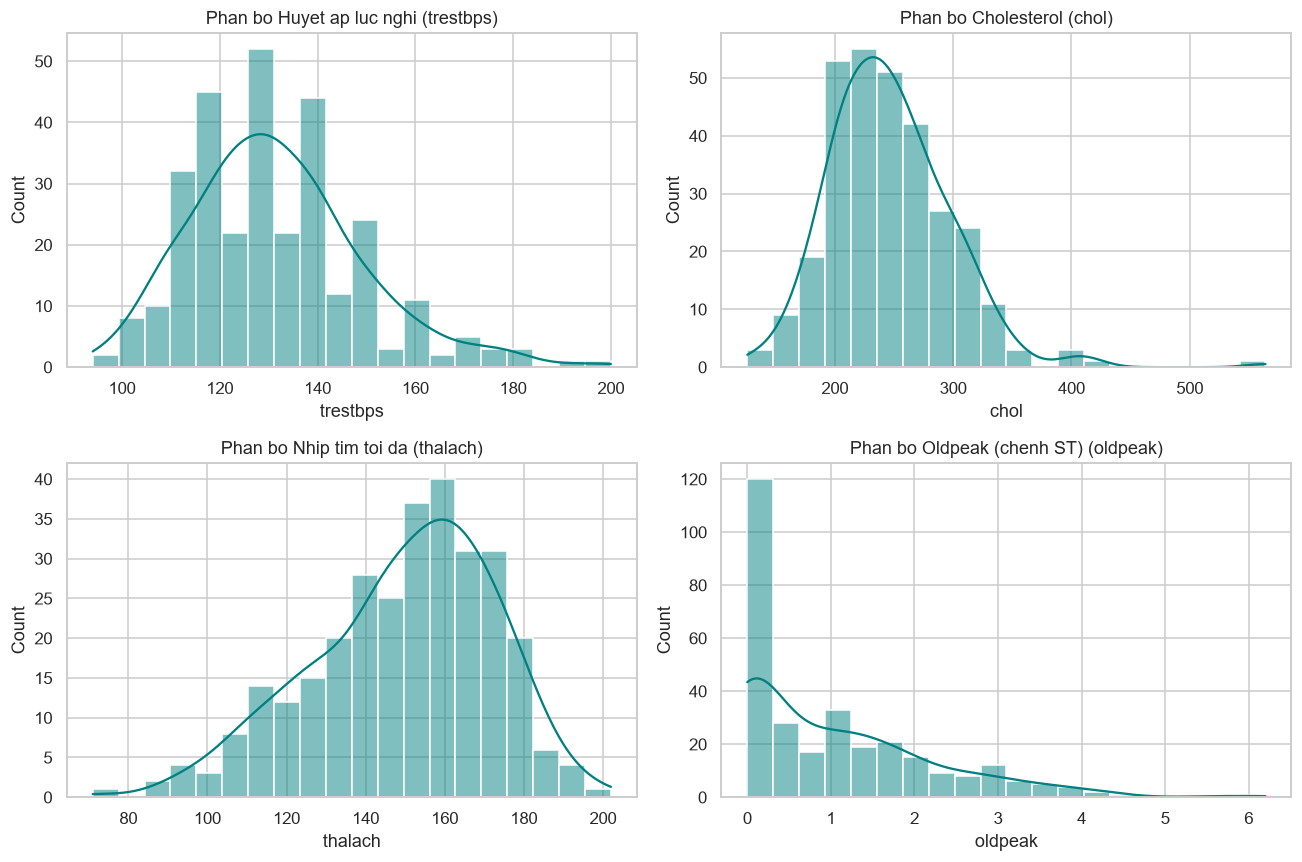
\includegraphics[width=\textwidth]{figures/continuous_histograms.png}
  \caption{Histogram các đặc trưng liên tục.}
  \label{fig:hist}
\end{figure}

\begin{figure}[h]
  \centering
  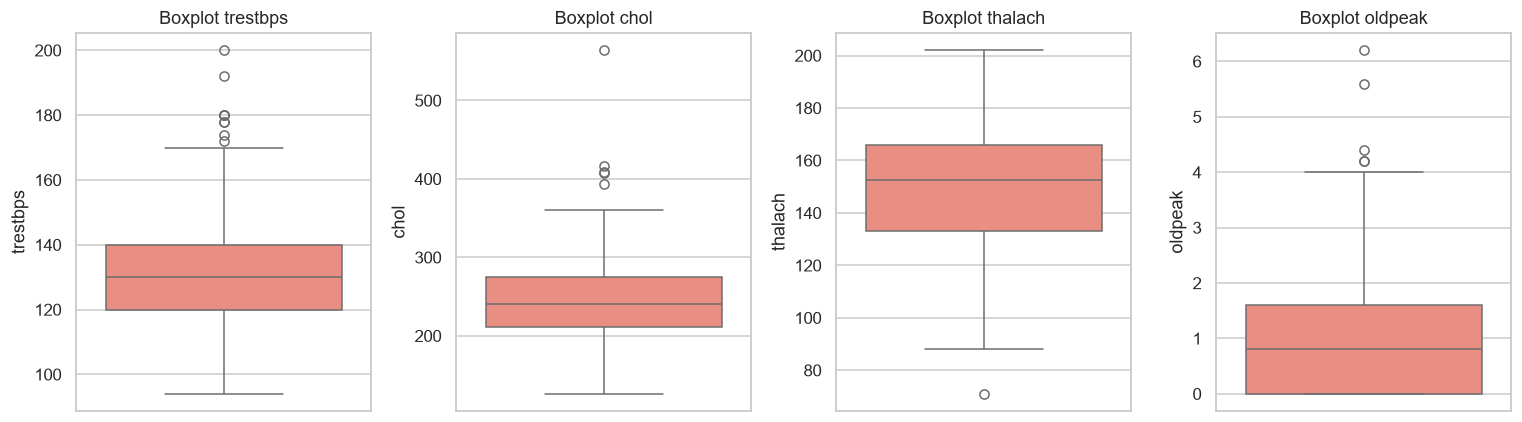
\includegraphics[width=\textwidth]{figures/continuous_boxplots.png}
  \caption{Boxplot các đặc trưng liên tục (quan sát outlier).}
  \label{fig:box}
\end{figure}

\begin{figure}[h]
  \centering
  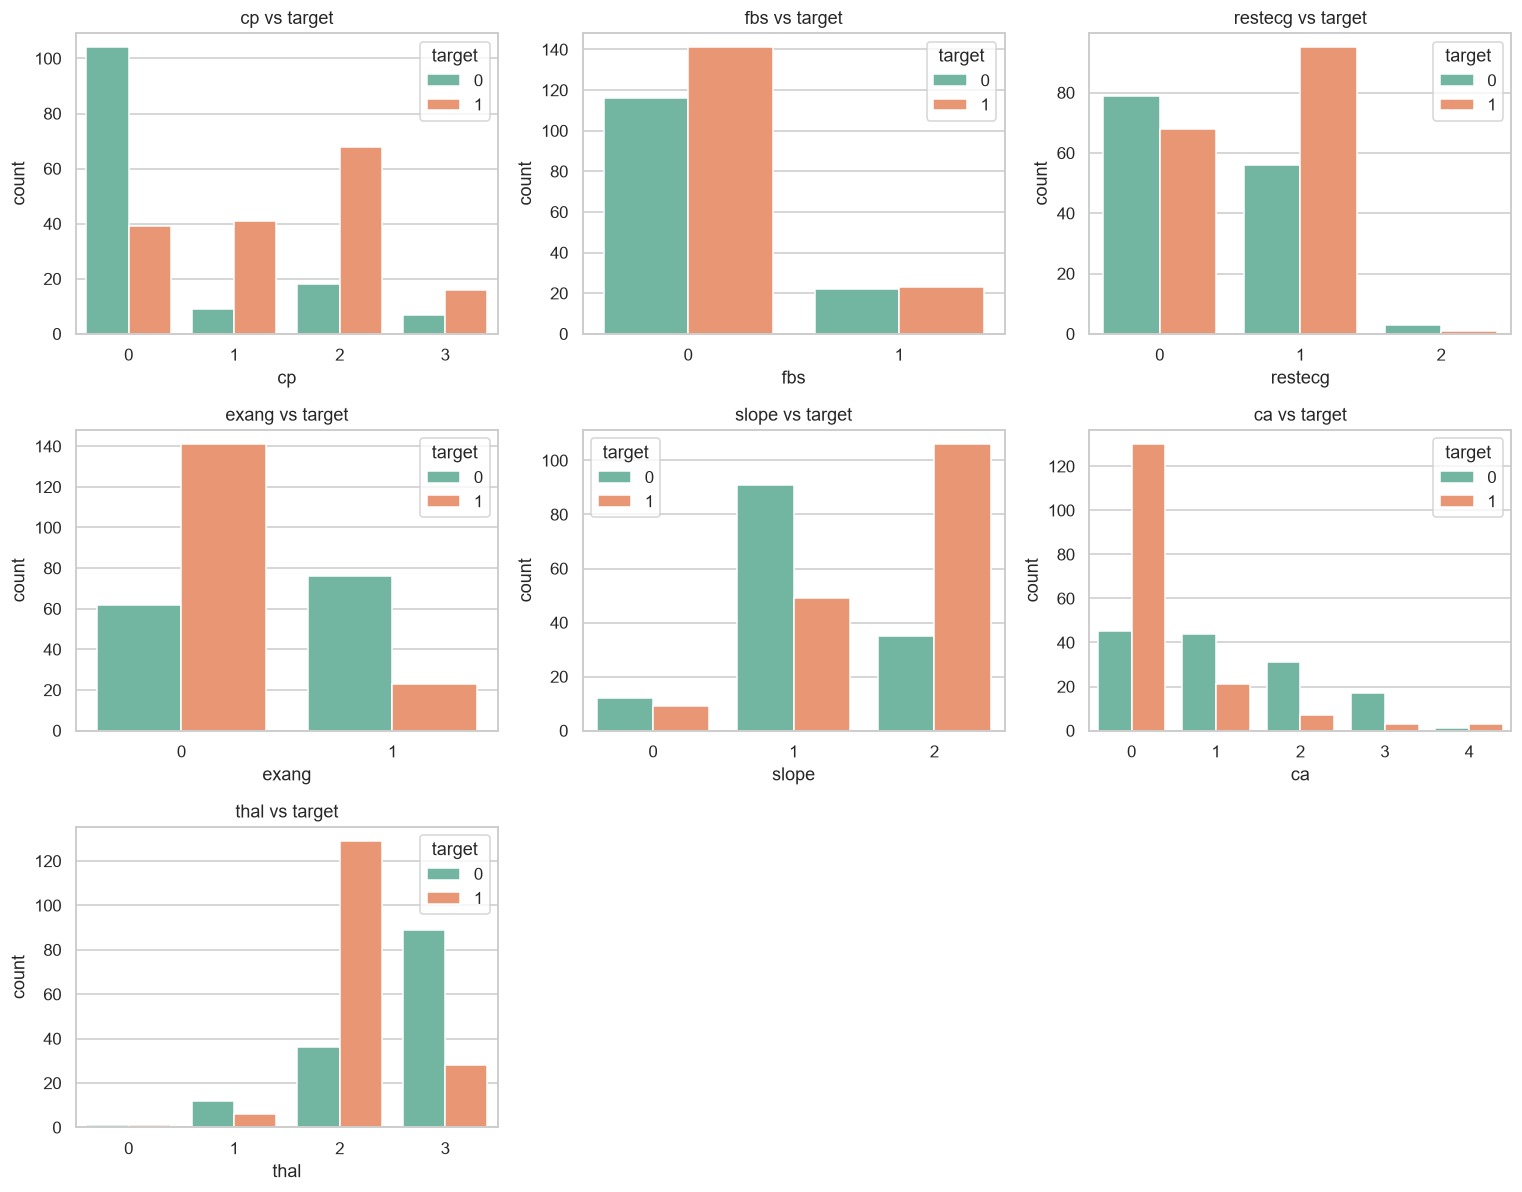
\includegraphics[width=\textwidth]{figures/categorical_countplots.png}
  \caption{Countplot các biến phân loại theo nhãn.}
  \label{fig:cat}
\end{figure}

\begin{figure}[h]
  \centering
  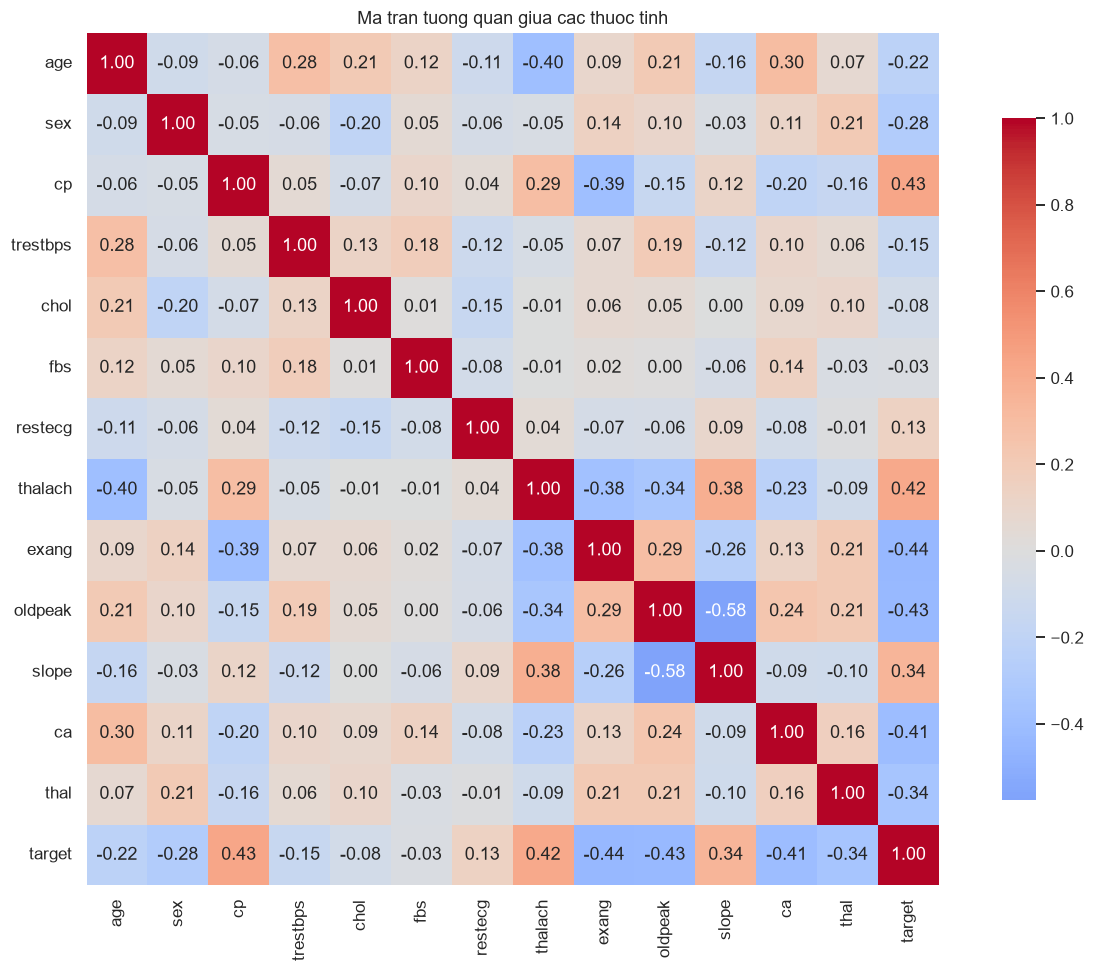
\includegraphics[width=0.9\textwidth]{figures/correlation_heatmap.png}
  \caption{Ma trận tương quan giữa các thuộc tính.}
  \label{fig:corr}
\end{figure}

\begin{table}[h]
\centering
\caption{Tương quan của từng thuộc tính với \texttt{target} (sắp theo độ lớn)}
\label{tab:corr}
\begin{tabular}{lc lc}
\toprule
Thuộc tính & Hệ số & Thuộc tính & Hệ số \\
\midrule
\texttt{exang}   & $-0.436$ & \texttt{thal}     & $-0.343$ \\
\texttt{cp}      & $+0.432$ & \texttt{sex}      & $-0.284$ \\
\texttt{oldpeak} & $-0.429$ & \texttt{age}      & $-0.221$ \\
\texttt{thalach} & $+0.420$ & \texttt{trestbps} & $-0.146$ \\
\texttt{ca}      & $-0.409$ & \texttt{restecg}  & $+0.135$ \\
\texttt{slope}   & $+0.344$ & \texttt{chol}     & $-0.081$ \\
                 &          & \texttt{fbs}      & $-0.027$ \\
\bottomrule
\end{tabular}
\end{table}

\textbf{Nhận xét:} các thuộc tính tương quan mạnh nhất với nguy cơ bệnh tim là
\texttt{exang}, \texttt{cp}, \texttt{oldpeak}, \texttt{thalach}, \texttt{ca},
phù hợp với y văn. Hai thuộc tính \texttt{chol} và \texttt{fbs} tương quan yếu
nhất với nhãn.

\section{Kết luận chương}
Chương 3 đã hoàn thành khâu chuẩn bị dữ liệu: làm sạch (loại 723 bản trùng còn
302 dòng, không có giá trị thiếu, xử lý outlier), chuẩn hoá đặc trưng bằng
\texttt{StandardScaler} (fit trên train để tránh rò rỉ dữ liệu), chia dữ liệu
80/20 có phân tầng và xuất \texttt{train.csv}/\texttt{test.csv}. EDA cho thấy dữ
liệu cân bằng nhãn và xác định được nhóm đặc trưng quan trọng. Bộ dữ liệu đã sẵn
sàng cho Chương 4 -- thiết kế và huấn luyện mô hình ANN.

% vao main.tex. Yeu cau goi cac package: graphicx, booktabs.
% Neu dung documentclass{article}, doi \chapter -> \section.
% =====================================================================

\chapter{Dữ liệu và tiền xử lý dữ liệu}
\label{chap:data}

\section{Giới thiệu bộ dữ liệu}
Bộ dữ liệu sử dụng là \textbf{Heart Disease Dataset} trên Kaggle
(\texttt{johnsmith88/heart-disease-dataset}), tổng hợp từ bốn cơ sở dữ liệu y tế
(Cleveland, Hungary, Switzerland, Long Beach V) từ năm 1988. Tuy bản gốc có 76
thuộc tính, các nghiên cứu công bố đều sử dụng tập con gồm \textbf{14 thuộc tính}.

\begin{itemize}
  \item Số bản ghi ban đầu: 1025 dòng.
  \item Số thuộc tính: 13 đặc trưng đầu vào và 1 biến mục tiêu \texttt{target}.
  \item Bài toán: phân loại nhị phân, dự đoán bệnh nhân \emph{có nguy cơ}
        (\texttt{target = 1}) hay \emph{không} (\texttt{target = 0}).
\end{itemize}

\begin{table}[h]
\centering
\caption{Mô tả các thuộc tính của bộ dữ liệu}
\label{tab:attributes}
\begin{tabular}{cllc}
\toprule
\# & Thuộc tính & Ý nghĩa & Kiểu \\
\midrule
1  & \texttt{age}      & Tuổi (năm)                              & Liên tục \\
2  & \texttt{sex}      & Giới tính (1 = nam, 0 = nữ)             & Nhị phân \\
3  & \texttt{cp}       & Kiểu đau ngực (0--3)                    & Phân loại \\
4  & \texttt{trestbps} & Huyết áp lúc nghỉ (mm Hg)               & Liên tục \\
5  & \texttt{chol}     & Cholesterol huyết thanh (mg/dl)         & Liên tục \\
6  & \texttt{fbs}      & Đường huyết đói $>$ 120 mg/dl (1/0)     & Nhị phân \\
7  & \texttt{restecg}  & Điện tâm đồ lúc nghỉ (0--2)             & Phân loại \\
8  & \texttt{thalach}  & Nhịp tim tối đa đạt được                & Liên tục \\
9  & \texttt{exang}    & Đau thắt ngực khi gắng sức (1/0)        & Nhị phân \\
10 & \texttt{oldpeak}  & Độ chênh đoạn ST khi gắng sức           & Liên tục \\
11 & \texttt{slope}    & Độ dốc đoạn ST khi gắng sức (0--2)      & Phân loại \\
12 & \texttt{ca}       & Số mạch máu lớn nhuộm màu (0--4)        & Phân loại \\
13 & \texttt{thal}     & Tình trạng thalassemia (0--3)           & Phân loại \\
14 & \texttt{target}   & Nhãn: 1 = có nguy cơ, 0 = không         & Nhị phân \\
\bottomrule
\end{tabular}
\end{table}

\section{Thống kê mô tả}
Các đặc trưng liên tục có thang đo rất khác nhau: \texttt{chol} ở mức hàng trăm
(126--564) trong khi \texttt{oldpeak} chỉ dao động 0--6.2. Do đó cần
\textbf{chuẩn hoá} trước khi đưa vào mạng nơ-ron (mục~\ref{sec:fe}).

\section{Kiểm tra chất lượng dữ liệu}

\subsection{Giá trị thiếu}
Kiểm tra bằng \texttt{df.isnull().sum()}: \textbf{không có ô thiếu}.

\subsection{Bản ghi trùng lặp}
Kiểm tra bằng \texttt{df.duplicated().sum()} cho thấy trong 1025 bản ghi có
\textbf{723 bản trùng lặp hoàn toàn}, chỉ còn \textbf{302 bản ghi duy nhất}.
Nếu giữ lại, một bệnh nhân có thể xuất hiện đồng thời ở cả tập train và test,
gây \textbf{rò rỉ dữ liệu (data leakage)} làm độ chính xác bị cao giả tạo. Vì
vậy nhóm loại bỏ toàn bộ bản trùng trước khi chia dữ liệu.

\subsection{Giá trị ngoại lệ (Outlier)}
Áp dụng quy tắc \textbf{IQR}: giá trị ngoài khoảng
$[Q_1 - 1.5\,\mathrm{IQR},\; Q_3 + 1.5\,\mathrm{IQR}]$ được coi là ngoại lệ.
Các outlier ở \texttt{trestbps}, \texttt{chol}, \texttt{thalach},
\texttt{oldpeak} được \textbf{cắt về biên} (winsorize) nhằm giảm nhiễu mà vẫn
giữ lại bản ghi.

\subsection{Giá trị bất thường về mã hoá}
\texttt{ca} có giá trị 4 và \texttt{thal} có giá trị 0 nằm ngoài bảng mã chuẩn;
do số lượng nhỏ, chúng được giữ lại như một mức phân loại riêng.

\section{Tiền xử lý dữ liệu}
Quy trình trong \texttt{src/data\_preprocessing.py}:
\begin{enumerate}
  \item Đọc dữ liệu thô \texttt{data/raw/heart.csv}.
  \item Loại bản ghi trùng: $1025 \rightarrow 302$ dòng.
  \item Điền giá trị thiếu (nếu có): liên tục dùng trung vị, phân loại dùng mode.
  \item Chuẩn hoá kiểu dữ liệu: cột phân loại/nhị phân về \texttt{int}, liên tục
        về \texttt{float}.
  \item Xử lý outlier bằng cách cắt về biên IQR.
  \item Lưu \texttt{data/processed/heart\_clean.csv} (302 dòng $\times$ 14 cột).
\end{enumerate}

\section{Feature Engineering}
\label{sec:fe}
Cài đặt trong \texttt{src/feature\_engineering.py}:
\begin{itemize}
  \item Mã hoá biến phân loại bằng \texttt{LabelEncoder} (giữ nguyên 13 đặc trưng
        để khớp lớp \texttt{Input(13)} của mô hình ANN).
  \item Chuẩn hoá đặc trưng liên tục bằng \texttt{StandardScaler} (trung bình 0,
        độ lệch chuẩn 1).
  \item Chống rò rỉ dữ liệu: \texttt{StandardScaler} chỉ \texttt{fit} trên tập
        train rồi áp dụng cho cả train và test; scaler được lưu tại
        \texttt{saved\_models/scaler.pkl}.
\end{itemize}

\section{Chia tập dữ liệu train/test}
Sử dụng \texttt{train\_test\_split()} với tỷ lệ \textbf{80\% train -- 20\% test},
\texttt{stratify} theo nhãn và \texttt{random\_state = 42}.

\begin{table}[h]
\centering
\caption{Kết quả chia tập dữ liệu}
\label{tab:split}
\begin{tabular}{lccc}
\toprule
Tập & Số mẫu & Nhãn 1 (có bệnh) & Nhãn 0 (không bệnh) \\
\midrule
Train & 241 & 131 & 110 \\
Test  & 61  & 33  & 28  \\
\midrule
Tổng  & 302 & 164 & 138 \\
\bottomrule
\end{tabular}
\end{table}

Kết quả lưu thành \texttt{data/processed/train.csv} và
\texttt{data/processed/test.csv}.

\section{Phân tích dữ liệu khám phá (EDA)}
EDA được thực hiện trong \texttt{notebook/data\_exploration.ipynb}.

\begin{figure}[h]
  \centering
  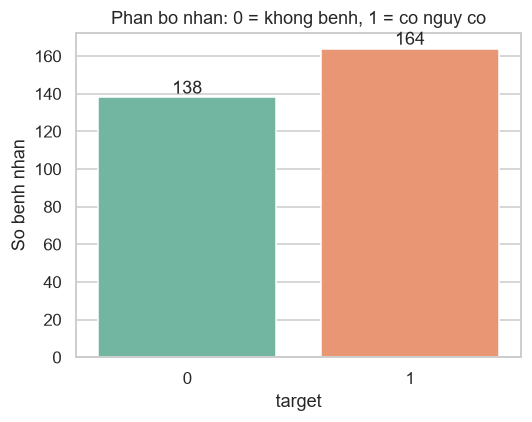
\includegraphics[width=0.5\textwidth]{figures/target_distribution.png}
  \caption{Phân bố biến mục tiêu \texttt{target} (cân bằng $\approx$ 54\%/46\%).}
  \label{fig:target}
\end{figure}

\begin{figure}[h]
  \centering
  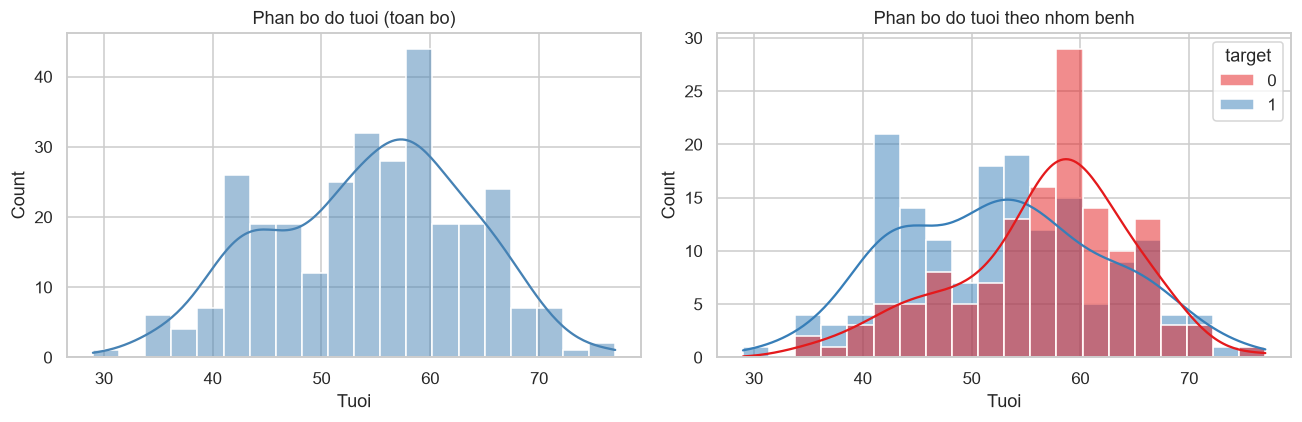
\includegraphics[width=\textwidth]{figures/age_distribution.png}
  \caption{Phân bố độ tuổi theo toàn bộ và theo nhóm bệnh.}
  \label{fig:age}
\end{figure}

\begin{figure}[h]
  \centering
  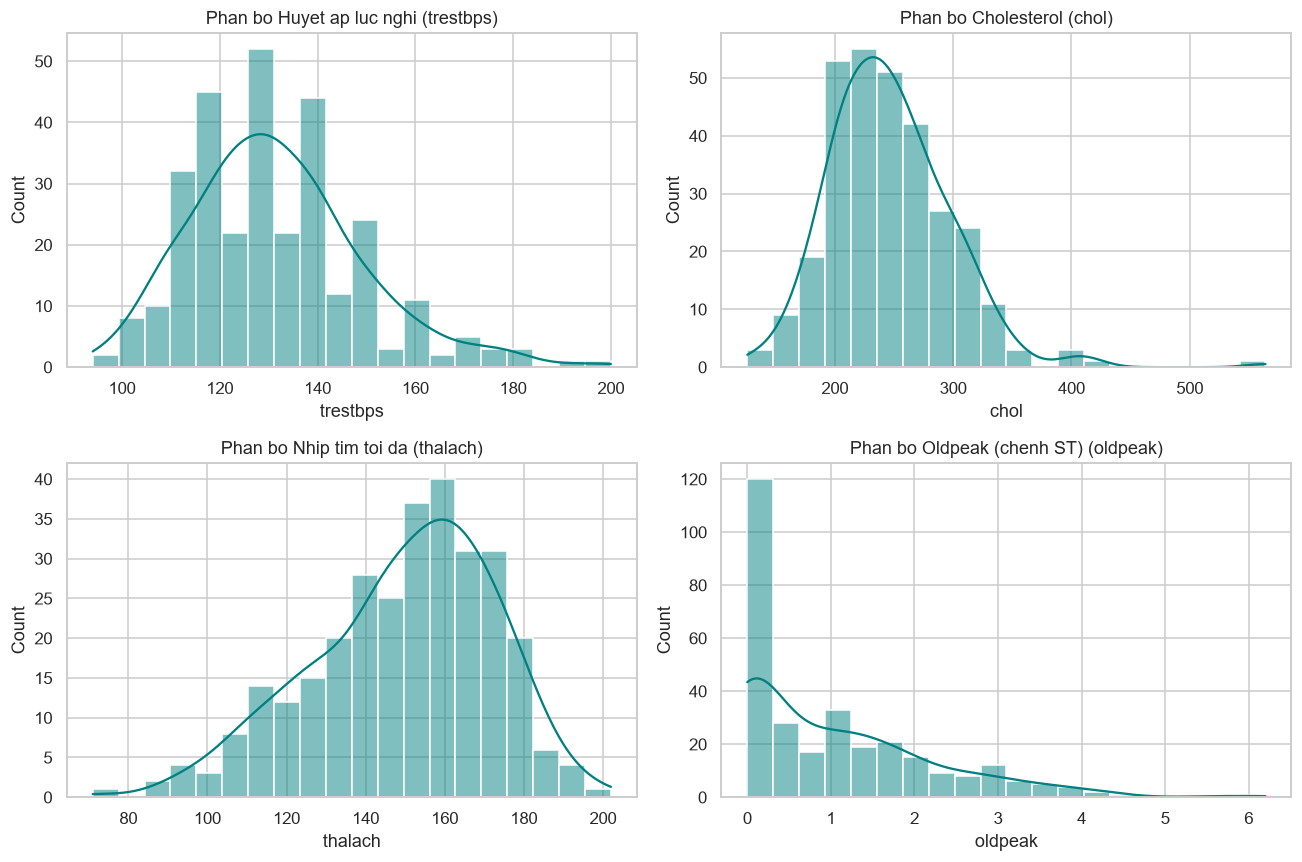
\includegraphics[width=\textwidth]{figures/continuous_histograms.png}
  \caption{Histogram các đặc trưng liên tục.}
  \label{fig:hist}
\end{figure}

\begin{figure}[h]
  \centering
  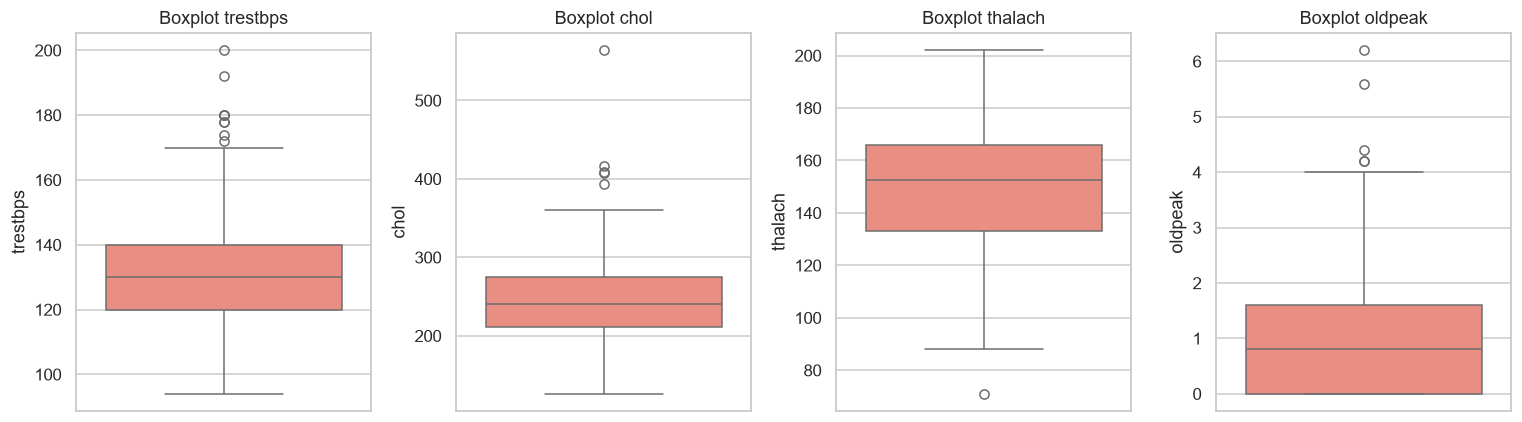
\includegraphics[width=\textwidth]{figures/continuous_boxplots.png}
  \caption{Boxplot các đặc trưng liên tục (quan sát outlier).}
  \label{fig:box}
\end{figure}

\begin{figure}[h]
  \centering
  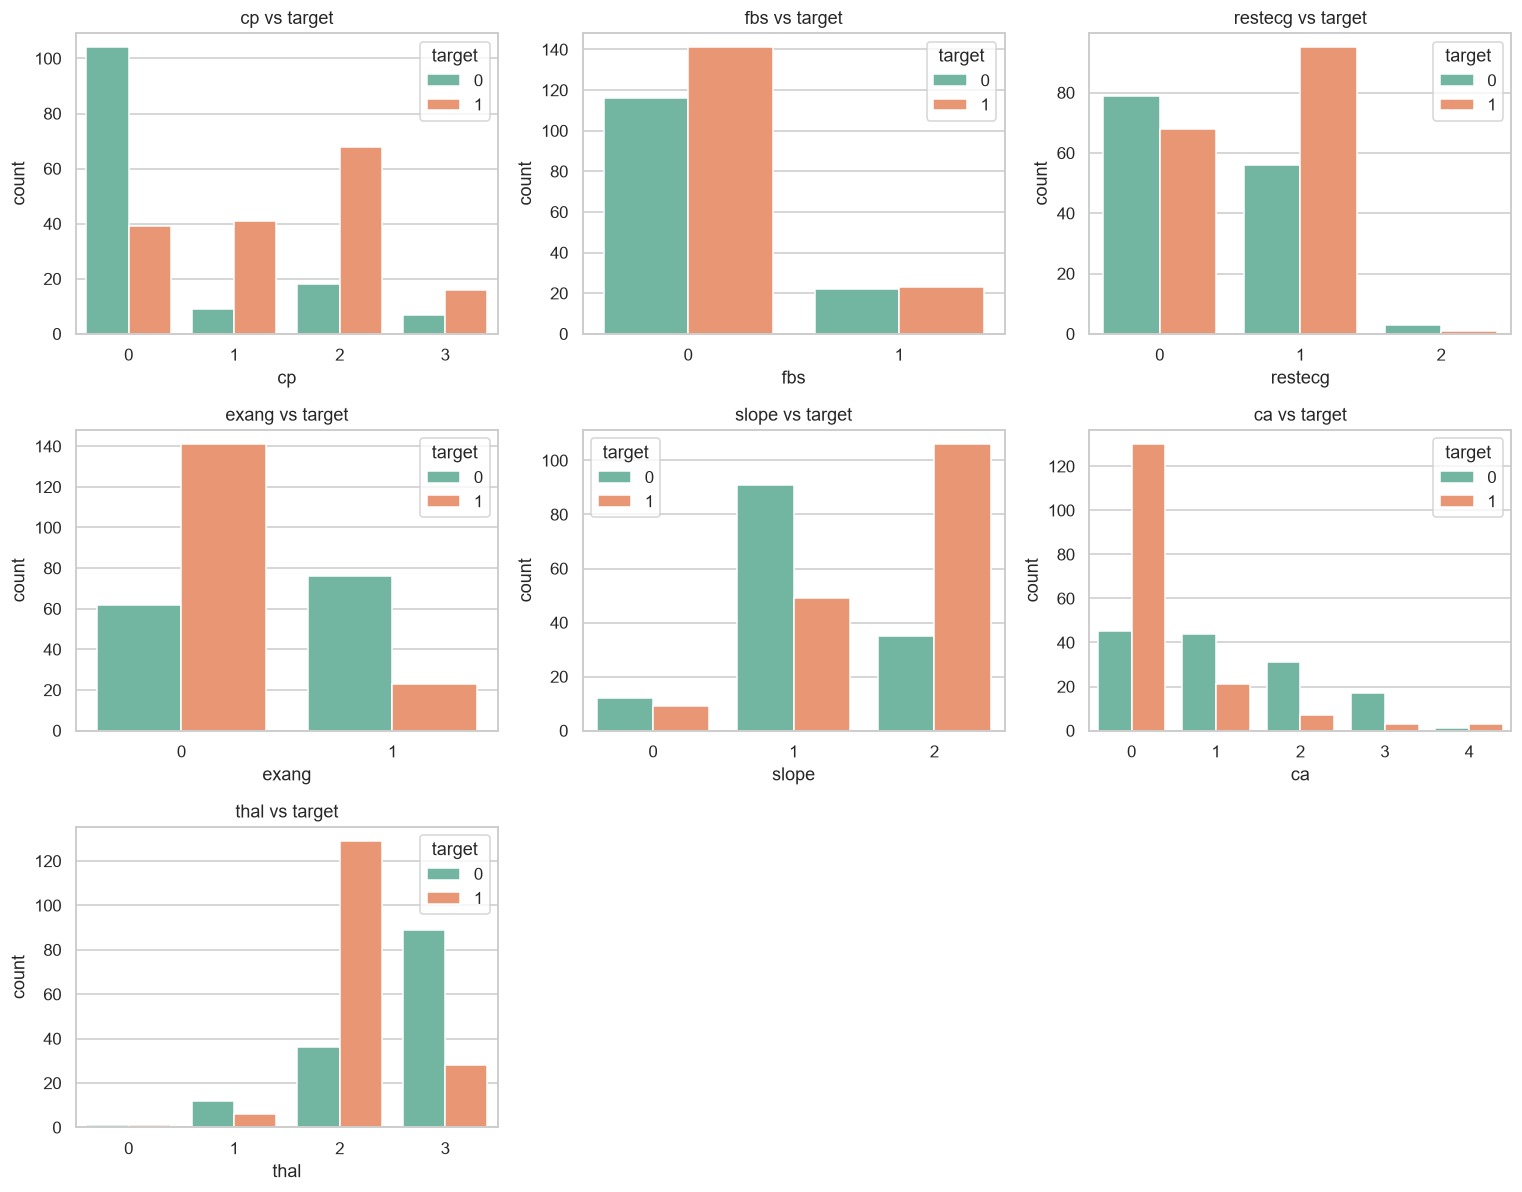
\includegraphics[width=\textwidth]{figures/categorical_countplots.png}
  \caption{Countplot các biến phân loại theo nhãn.}
  \label{fig:cat}
\end{figure}

\begin{figure}[h]
  \centering
  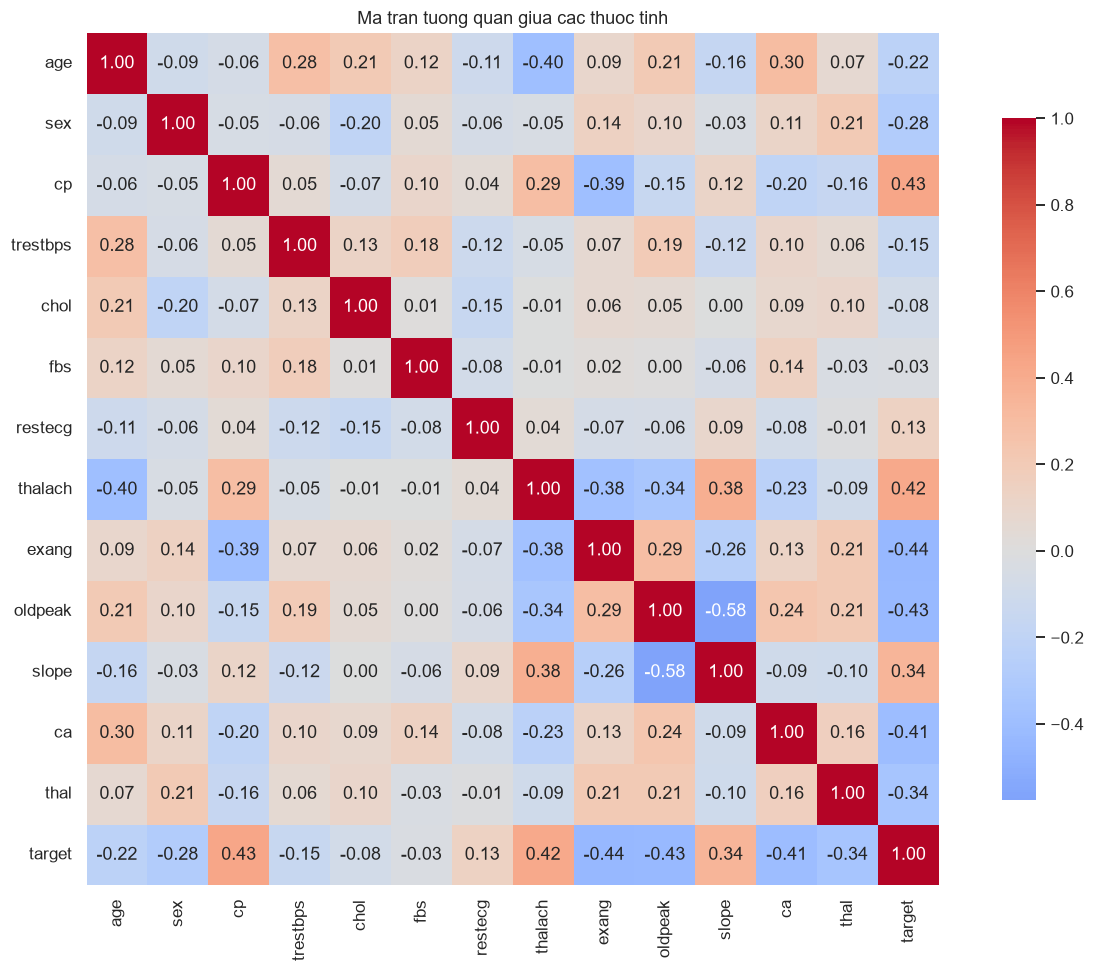
\includegraphics[width=0.9\textwidth]{figures/correlation_heatmap.png}
  \caption{Ma trận tương quan giữa các thuộc tính.}
  \label{fig:corr}
\end{figure}

\begin{table}[h]
\centering
\caption{Tương quan của từng thuộc tính với \texttt{target} (sắp theo độ lớn)}
\label{tab:corr}
\begin{tabular}{lc lc}
\toprule
Thuộc tính & Hệ số & Thuộc tính & Hệ số \\
\midrule
\texttt{exang}   & $-0.436$ & \texttt{thal}     & $-0.343$ \\
\texttt{cp}      & $+0.432$ & \texttt{sex}      & $-0.284$ \\
\texttt{oldpeak} & $-0.429$ & \texttt{age}      & $-0.221$ \\
\texttt{thalach} & $+0.420$ & \texttt{trestbps} & $-0.146$ \\
\texttt{ca}      & $-0.409$ & \texttt{restecg}  & $+0.135$ \\
\texttt{slope}   & $+0.344$ & \texttt{chol}     & $-0.081$ \\
                 &          & \texttt{fbs}      & $-0.027$ \\
\bottomrule
\end{tabular}
\end{table}

\textbf{Nhận xét:} các thuộc tính tương quan mạnh nhất với nguy cơ bệnh tim là
\texttt{exang}, \texttt{cp}, \texttt{oldpeak}, \texttt{thalach}, \texttt{ca},
phù hợp với y văn. Hai thuộc tính \texttt{chol} và \texttt{fbs} tương quan yếu
nhất với nhãn.

\section{Kết luận chương}
Chương 3 đã hoàn thành khâu chuẩn bị dữ liệu: làm sạch (loại 723 bản trùng còn
302 dòng, không có giá trị thiếu, xử lý outlier), chuẩn hoá đặc trưng bằng
\texttt{StandardScaler} (fit trên train để tránh rò rỉ dữ liệu), chia dữ liệu
80/20 có phân tầng và xuất \texttt{train.csv}/\texttt{test.csv}. EDA cho thấy dữ
liệu cân bằng nhãn và xác định được nhóm đặc trưng quan trọng. Bộ dữ liệu đã sẵn
sàng cho Chương 4 -- thiết kế và huấn luyện mô hình ANN.

% vao main.tex. Yeu cau goi cac package: graphicx, booktabs.
% Neu dung documentclass{article}, doi \chapter -> \section.
% =====================================================================

\chapter{Dữ liệu và tiền xử lý dữ liệu}
\label{chap:data}

\section{Giới thiệu bộ dữ liệu}
Bộ dữ liệu sử dụng là \textbf{Heart Disease Dataset} trên Kaggle
(\texttt{johnsmith88/heart-disease-dataset}), tổng hợp từ bốn cơ sở dữ liệu y tế
(Cleveland, Hungary, Switzerland, Long Beach V) từ năm 1988. Tuy bản gốc có 76
thuộc tính, các nghiên cứu công bố đều sử dụng tập con gồm \textbf{14 thuộc tính}.

\begin{itemize}
  \item Số bản ghi ban đầu: 1025 dòng.
  \item Số thuộc tính: 13 đặc trưng đầu vào và 1 biến mục tiêu \texttt{target}.
  \item Bài toán: phân loại nhị phân, dự đoán bệnh nhân \emph{có nguy cơ}
        (\texttt{target = 1}) hay \emph{không} (\texttt{target = 0}).
\end{itemize}

\begin{table}[h]
\centering
\caption{Mô tả các thuộc tính của bộ dữ liệu}
\label{tab:attributes}
\begin{tabular}{cllc}
\toprule
\# & Thuộc tính & Ý nghĩa & Kiểu \\
\midrule
1  & \texttt{age}      & Tuổi (năm)                              & Liên tục \\
2  & \texttt{sex}      & Giới tính (1 = nam, 0 = nữ)             & Nhị phân \\
3  & \texttt{cp}       & Kiểu đau ngực (0--3)                    & Phân loại \\
4  & \texttt{trestbps} & Huyết áp lúc nghỉ (mm Hg)               & Liên tục \\
5  & \texttt{chol}     & Cholesterol huyết thanh (mg/dl)         & Liên tục \\
6  & \texttt{fbs}      & Đường huyết đói $>$ 120 mg/dl (1/0)     & Nhị phân \\
7  & \texttt{restecg}  & Điện tâm đồ lúc nghỉ (0--2)             & Phân loại \\
8  & \texttt{thalach}  & Nhịp tim tối đa đạt được                & Liên tục \\
9  & \texttt{exang}    & Đau thắt ngực khi gắng sức (1/0)        & Nhị phân \\
10 & \texttt{oldpeak}  & Độ chênh đoạn ST khi gắng sức           & Liên tục \\
11 & \texttt{slope}    & Độ dốc đoạn ST khi gắng sức (0--2)      & Phân loại \\
12 & \texttt{ca}       & Số mạch máu lớn nhuộm màu (0--4)        & Phân loại \\
13 & \texttt{thal}     & Tình trạng thalassemia (0--3)           & Phân loại \\
14 & \texttt{target}   & Nhãn: 1 = có nguy cơ, 0 = không         & Nhị phân \\
\bottomrule
\end{tabular}
\end{table}

\section{Thống kê mô tả}
Các đặc trưng liên tục có thang đo rất khác nhau: \texttt{chol} ở mức hàng trăm
(126--564) trong khi \texttt{oldpeak} chỉ dao động 0--6.2. Do đó cần
\textbf{chuẩn hoá} trước khi đưa vào mạng nơ-ron (mục~\ref{sec:fe}).

\section{Kiểm tra chất lượng dữ liệu}

\subsection{Giá trị thiếu}
Kiểm tra bằng \texttt{df.isnull().sum()}: \textbf{không có ô thiếu}.

\subsection{Bản ghi trùng lặp}
Kiểm tra bằng \texttt{df.duplicated().sum()} cho thấy trong 1025 bản ghi có
\textbf{723 bản trùng lặp hoàn toàn}, chỉ còn \textbf{302 bản ghi duy nhất}.
Nếu giữ lại, một bệnh nhân có thể xuất hiện đồng thời ở cả tập train và test,
gây \textbf{rò rỉ dữ liệu (data leakage)} làm độ chính xác bị cao giả tạo. Vì
vậy nhóm loại bỏ toàn bộ bản trùng trước khi chia dữ liệu.

\subsection{Giá trị ngoại lệ (Outlier)}
Áp dụng quy tắc \textbf{IQR}: giá trị ngoài khoảng
$[Q_1 - 1.5\,\mathrm{IQR},\; Q_3 + 1.5\,\mathrm{IQR}]$ được coi là ngoại lệ.
Các outlier ở \texttt{trestbps}, \texttt{chol}, \texttt{thalach},
\texttt{oldpeak} được \textbf{cắt về biên} (winsorize) nhằm giảm nhiễu mà vẫn
giữ lại bản ghi.

\subsection{Giá trị bất thường về mã hoá}
\texttt{ca} có giá trị 4 và \texttt{thal} có giá trị 0 nằm ngoài bảng mã chuẩn;
do số lượng nhỏ, chúng được giữ lại như một mức phân loại riêng.

\section{Tiền xử lý dữ liệu}
Quy trình trong \texttt{src/data\_preprocessing.py}:
\begin{enumerate}
  \item Đọc dữ liệu thô \texttt{data/raw/heart.csv}.
  \item Loại bản ghi trùng: $1025 \rightarrow 302$ dòng.
  \item Điền giá trị thiếu (nếu có): liên tục dùng trung vị, phân loại dùng mode.
  \item Chuẩn hoá kiểu dữ liệu: cột phân loại/nhị phân về \texttt{int}, liên tục
        về \texttt{float}.
  \item Xử lý outlier bằng cách cắt về biên IQR.
  \item Lưu \texttt{data/processed/heart\_clean.csv} (302 dòng $\times$ 14 cột).
\end{enumerate}

\section{Feature Engineering}
\label{sec:fe}
Cài đặt trong \texttt{src/feature\_engineering.py}:
\begin{itemize}
  \item Mã hoá biến phân loại bằng \texttt{LabelEncoder} (giữ nguyên 13 đặc trưng
        để khớp lớp \texttt{Input(13)} của mô hình ANN).
  \item Chuẩn hoá đặc trưng liên tục bằng \texttt{StandardScaler} (trung bình 0,
        độ lệch chuẩn 1).
  \item Chống rò rỉ dữ liệu: \texttt{StandardScaler} chỉ \texttt{fit} trên tập
        train rồi áp dụng cho cả train và test; scaler được lưu tại
        \texttt{saved\_models/scaler.pkl}.
\end{itemize}

\section{Chia tập dữ liệu train/test}
Sử dụng \texttt{train\_test\_split()} với tỷ lệ \textbf{80\% train -- 20\% test},
\texttt{stratify} theo nhãn và \texttt{random\_state = 42}.

\begin{table}[h]
\centering
\caption{Kết quả chia tập dữ liệu}
\label{tab:split}
\begin{tabular}{lccc}
\toprule
Tập & Số mẫu & Nhãn 1 (có bệnh) & Nhãn 0 (không bệnh) \\
\midrule
Train & 241 & 131 & 110 \\
Test  & 61  & 33  & 28  \\
\midrule
Tổng  & 302 & 164 & 138 \\
\bottomrule
\end{tabular}
\end{table}

Kết quả lưu thành \texttt{data/processed/train.csv} và
\texttt{data/processed/test.csv}.

\section{Phân tích dữ liệu khám phá (EDA)}
EDA được thực hiện trong \texttt{notebook/data\_exploration.ipynb}.

\begin{figure}[h]
  \centering
  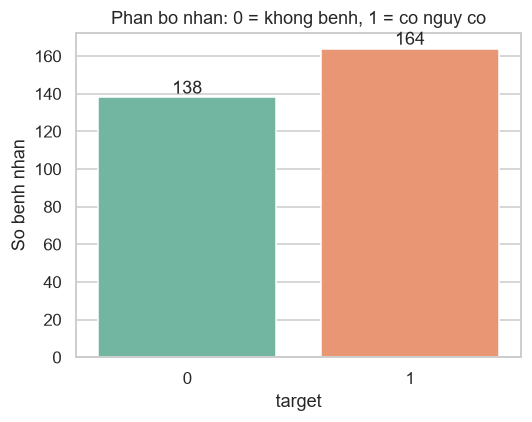
\includegraphics[width=0.5\textwidth]{figures/target_distribution.png}
  \caption{Phân bố biến mục tiêu \texttt{target} (cân bằng $\approx$ 54\%/46\%).}
  \label{fig:target}
\end{figure}

\begin{figure}[h]
  \centering
  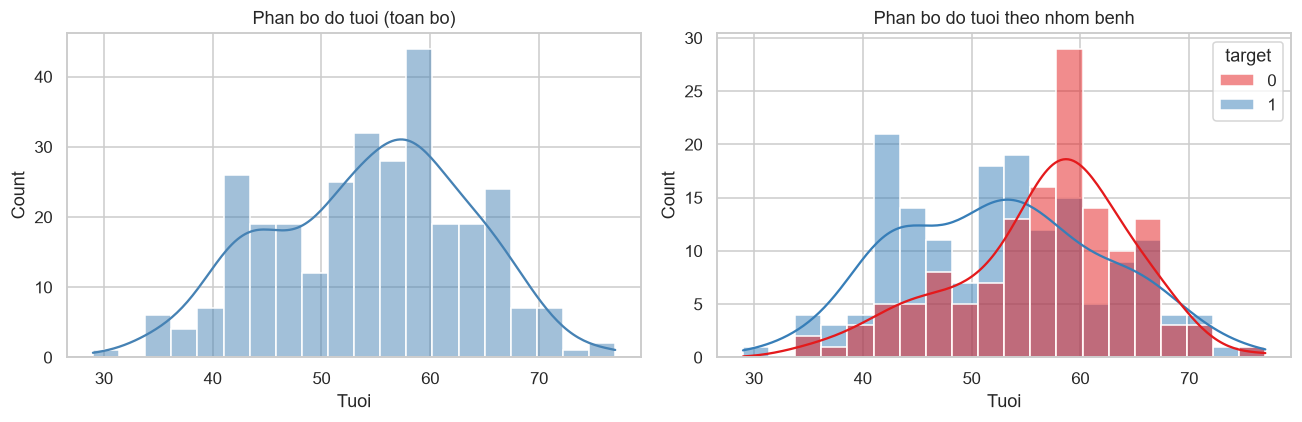
\includegraphics[width=\textwidth]{figures/age_distribution.png}
  \caption{Phân bố độ tuổi theo toàn bộ và theo nhóm bệnh.}
  \label{fig:age}
\end{figure}

\begin{figure}[h]
  \centering
  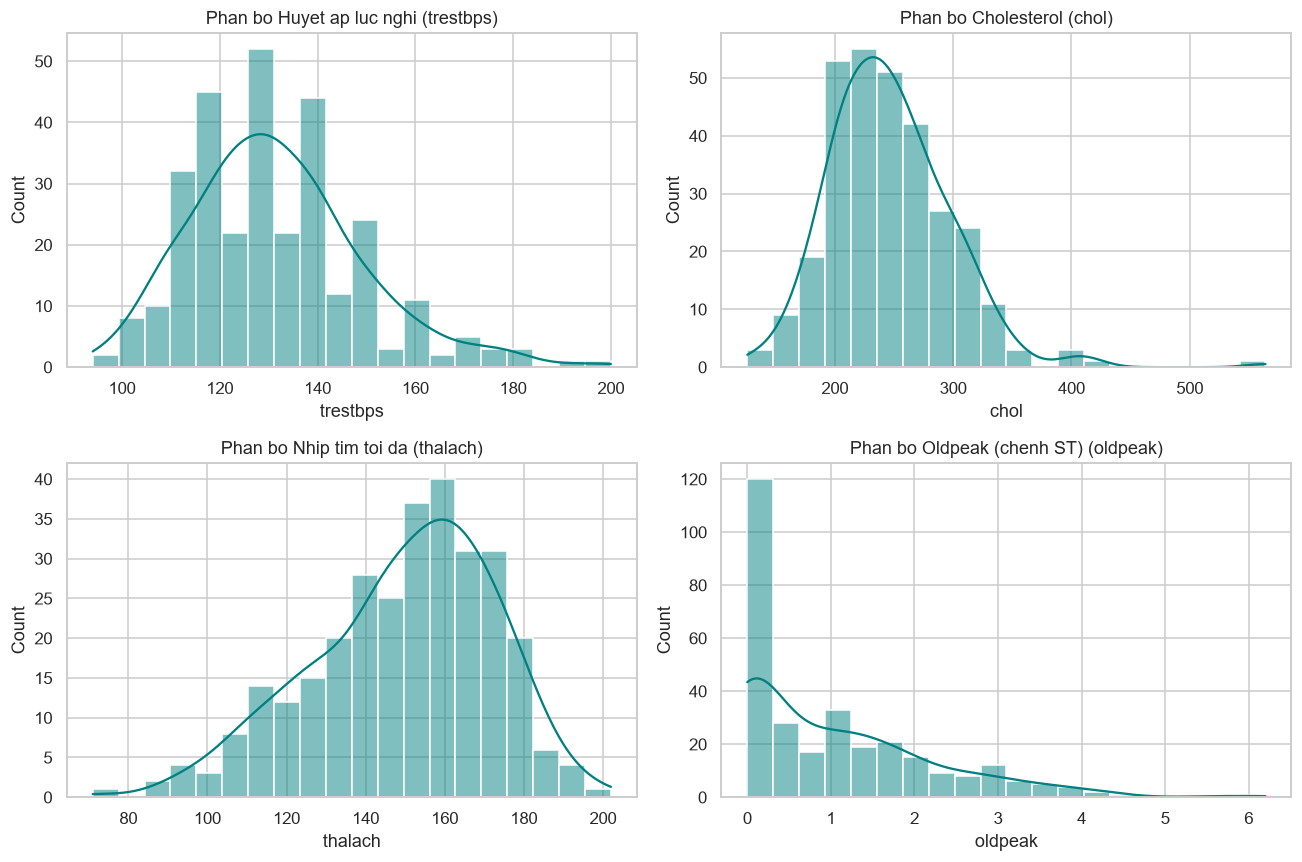
\includegraphics[width=\textwidth]{figures/continuous_histograms.png}
  \caption{Histogram các đặc trưng liên tục.}
  \label{fig:hist}
\end{figure}

\begin{figure}[h]
  \centering
  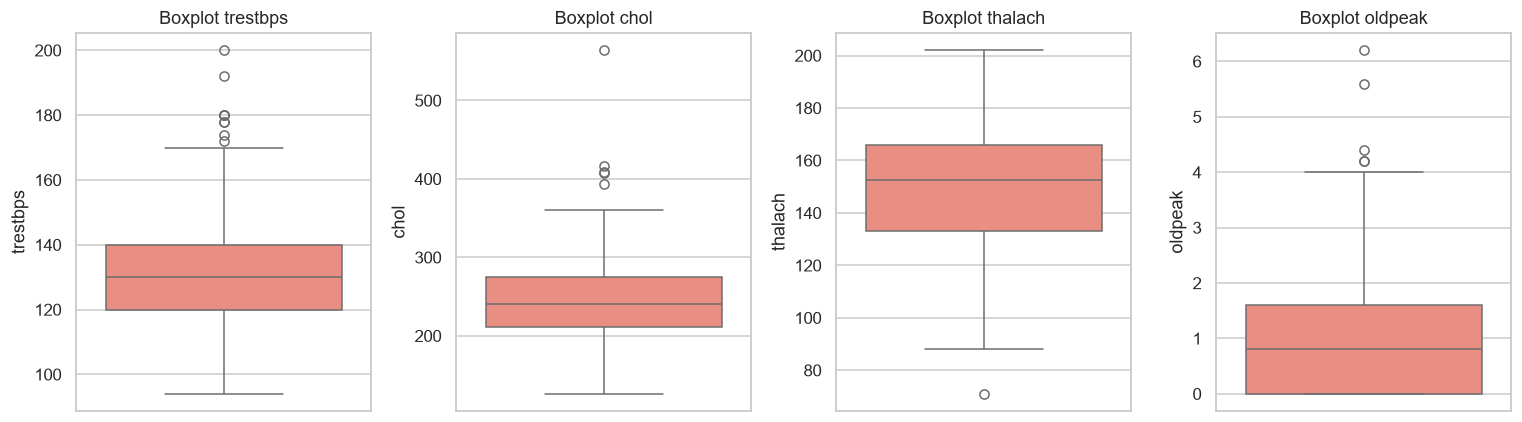
\includegraphics[width=\textwidth]{figures/continuous_boxplots.png}
  \caption{Boxplot các đặc trưng liên tục (quan sát outlier).}
  \label{fig:box}
\end{figure}

\begin{figure}[h]
  \centering
  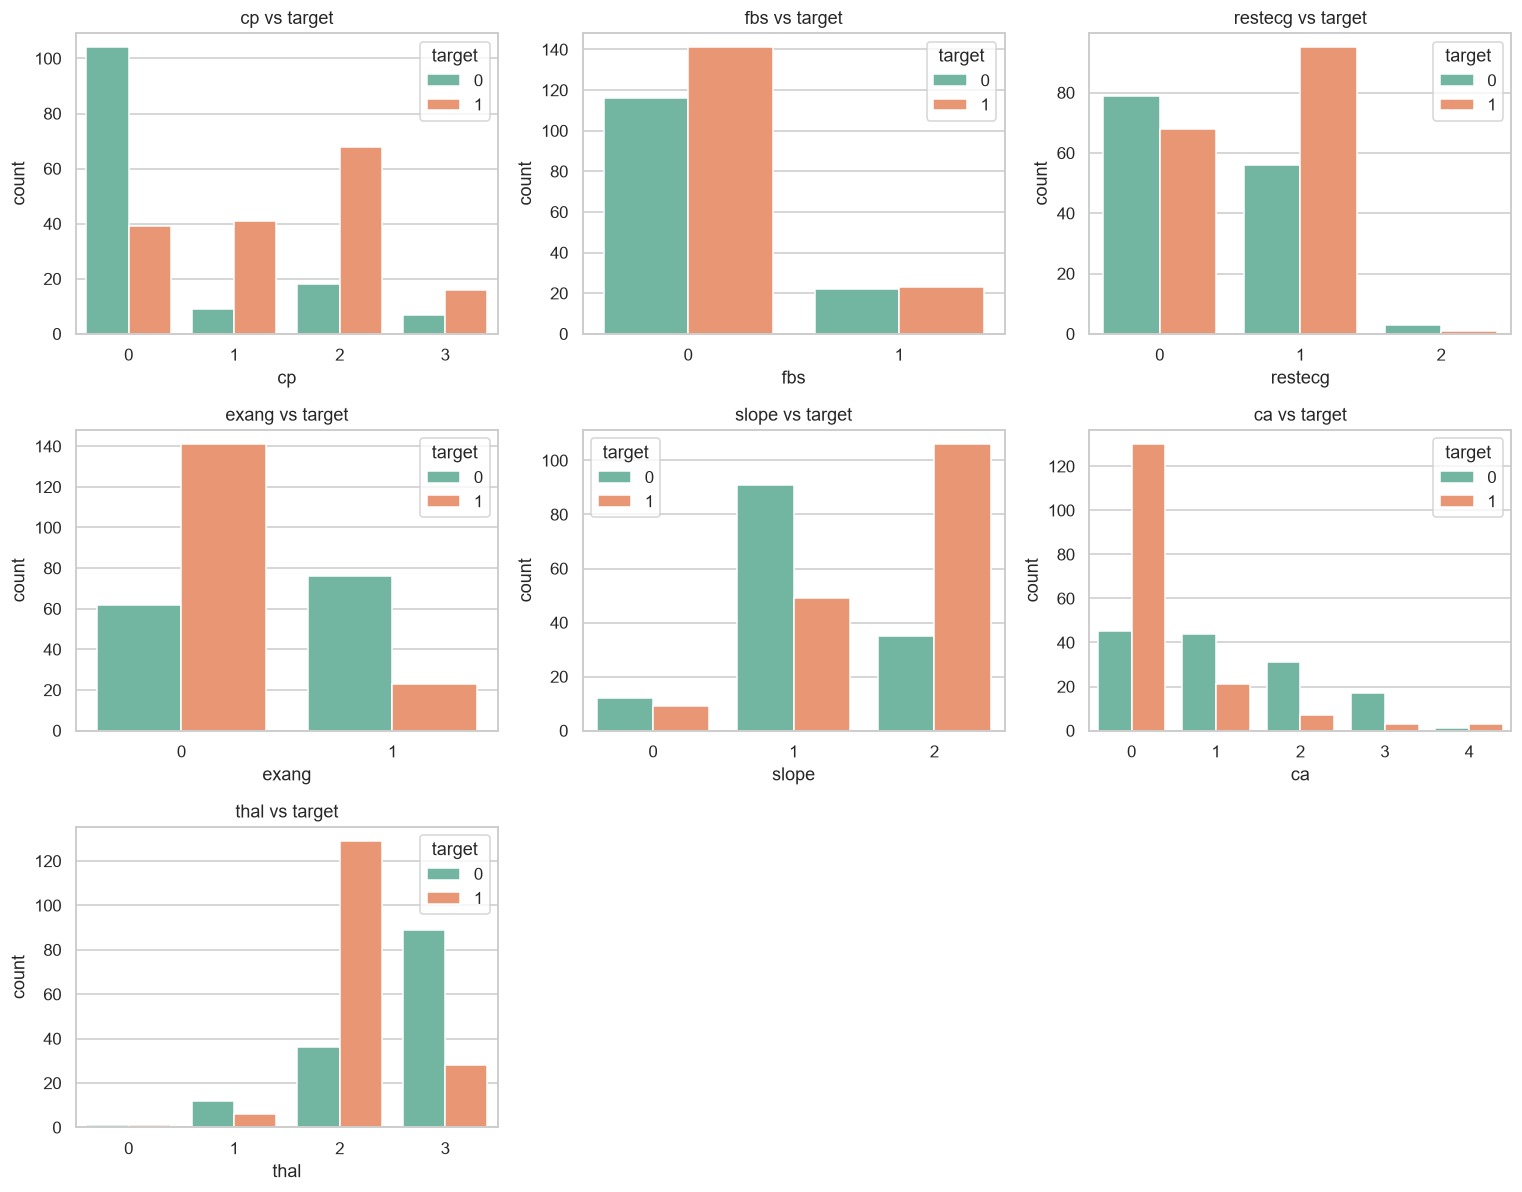
\includegraphics[width=\textwidth]{figures/categorical_countplots.png}
  \caption{Countplot các biến phân loại theo nhãn.}
  \label{fig:cat}
\end{figure}

\begin{figure}[h]
  \centering
  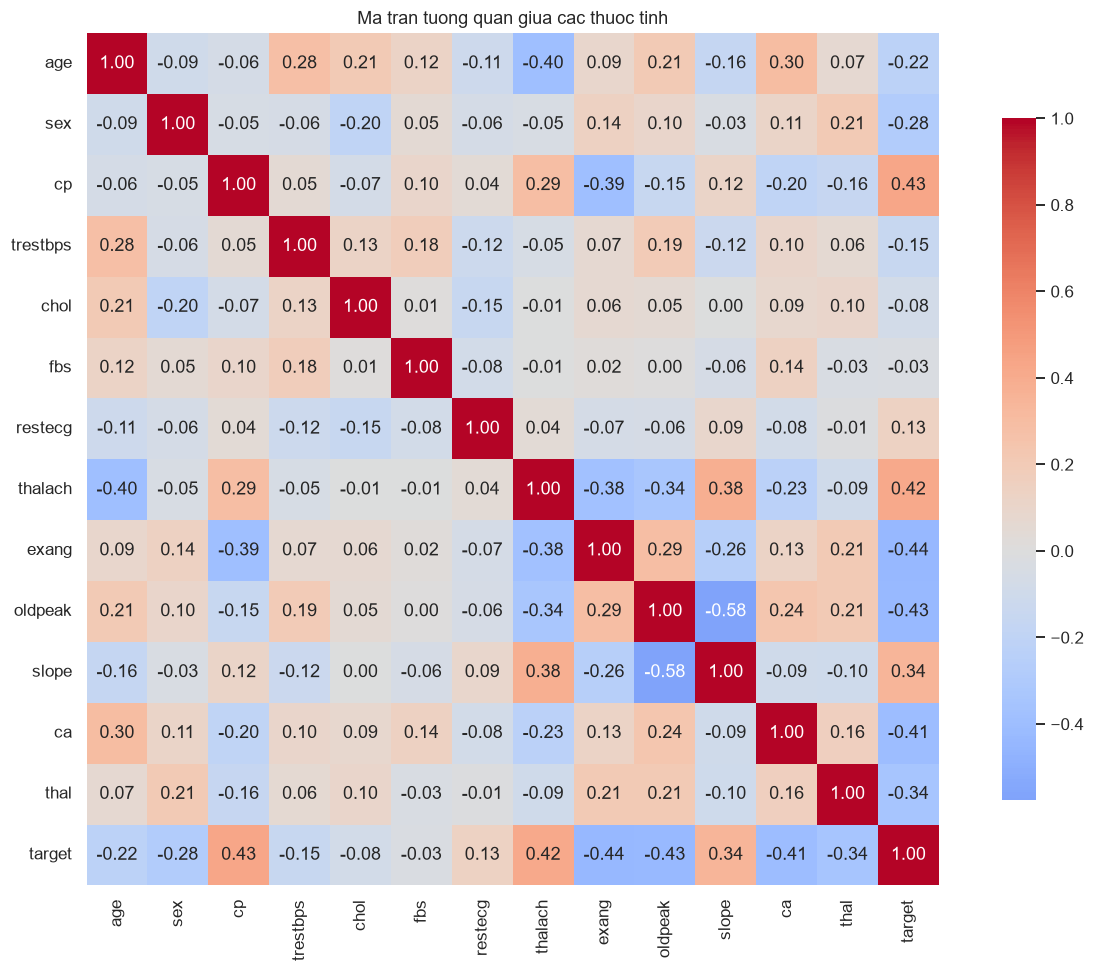
\includegraphics[width=0.9\textwidth]{figures/correlation_heatmap.png}
  \caption{Ma trận tương quan giữa các thuộc tính.}
  \label{fig:corr}
\end{figure}

\begin{table}[h]
\centering
\caption{Tương quan của từng thuộc tính với \texttt{target} (sắp theo độ lớn)}
\label{tab:corr}
\begin{tabular}{lc lc}
\toprule
Thuộc tính & Hệ số & Thuộc tính & Hệ số \\
\midrule
\texttt{exang}   & $-0.436$ & \texttt{thal}     & $-0.343$ \\
\texttt{cp}      & $+0.432$ & \texttt{sex}      & $-0.284$ \\
\texttt{oldpeak} & $-0.429$ & \texttt{age}      & $-0.221$ \\
\texttt{thalach} & $+0.420$ & \texttt{trestbps} & $-0.146$ \\
\texttt{ca}      & $-0.409$ & \texttt{restecg}  & $+0.135$ \\
\texttt{slope}   & $+0.344$ & \texttt{chol}     & $-0.081$ \\
                 &          & \texttt{fbs}      & $-0.027$ \\
\bottomrule
\end{tabular}
\end{table}

\textbf{Nhận xét:} các thuộc tính tương quan mạnh nhất với nguy cơ bệnh tim là
\texttt{exang}, \texttt{cp}, \texttt{oldpeak}, \texttt{thalach}, \texttt{ca},
phù hợp với y văn. Hai thuộc tính \texttt{chol} và \texttt{fbs} tương quan yếu
nhất với nhãn.

\section{Kết luận chương}
Chương 3 đã hoàn thành khâu chuẩn bị dữ liệu: làm sạch (loại 723 bản trùng còn
302 dòng, không có giá trị thiếu, xử lý outlier), chuẩn hoá đặc trưng bằng
\texttt{StandardScaler} (fit trên train để tránh rò rỉ dữ liệu), chia dữ liệu
80/20 có phân tầng và xuất \texttt{train.csv}/\texttt{test.csv}. EDA cho thấy dữ
liệu cân bằng nhãn và xác định được nhóm đặc trưng quan trọng. Bộ dữ liệu đã sẵn
sàng cho Chương 4 -- thiết kế và huấn luyện mô hình ANN.
